\documentclass[twoside]{esi-tfg}
\usepackage{custom}
\usepackage{epigraph}

%% -- Información general --
\title{Alcaudon: Streaming data platform}
\author{Francisco Fernández Castaño}{}


%% -- Variables de la clase esi-tfg --

%- datos del autor

%\address{}
%\city{}
%\country{}
\email{francisco.fernandez.castano@gmail.com}
\phone{645999999}
% \homepage{http://esi.uclm.es/~juan.nadie}


%- datos del documento

%\logo{informatica.pdf}
\advisorFirst{Dr. David Villa Alises}
\advisorDepartment{Departamento de Tecnologías y Sistemas de la Información}

\docdate{2017}{September}
\intensification{Computation}
%\license{Texto de licencia al gusto de cada uno.}


\begin{document}

\cover
\bastardtitle
\frontpage

\frontmatter
\copyrightpage
\jury

\selectlanguage{spanish}
\chapter{Resumen}

En los últimos años, la cantidad de datos recolectados no ha parado de crecer.
Las empresas de internet registran todas las acciones de sus usuarios para
proveer mejores experiencias. Los experimentos científicos generan grandes
cantidades de datos. El auge del \textit{Internet de las Cosas} ha traido
consigo un aumento de los datos a almacenar, por ejemplo los coches autónomos
necesitan analizar grandes cantidades de información para funcionar
correctamente. Estos hechos, combinados con el decreciente coste del
almacenamiento de datos, ha hecho que distintas organizaciones aprecien el
potencial de sus datos y busquen distintas formas de analizarlos.

Las empresas deben ganar ventaja competitiva usando sus datos a la hora de tomar
decisiones en lugar de basar las mismas en intuiciones. Debido a esta tendencia,
diversos sistemas para el análisis de grandes cantidades de datos han surgido en
los últimos años. Esos sistemas fueron diseñados para analizar grandes
cantidades de datos históricos. Sin embargo, en los últimos tiempos se está
dando una creciente necesidad de extraer conocimiento de los datos tan pronto
como sea posible. Esto ayuda a las organizaciones a reaccionar de una forma ágil
ante eventos de divérsa índole.

Este proyecto, Alcaudon, tiene como objetivo implementar un sistema de análisis
distribuido para datos en \textit{streaming}. Alcaudon permitirá analizar
fuentes de datos infinitas en \textit{tiempo real}. Uno de los objetivos de este
proyecto es proveer un modelo de programación para la creación de computaciones
distribuidas, facilitando la creación de \textit{pipelines} para el análisis de
datos en \textit{streaming}. Además, Alcaudon ha sido diseñado teniendo en
cuenta criterios de escalabilidad y tolerancia a fallos. Por tanto, este
proyecto presenta una herramienta robusta y potente para el procesado y análisis
de fuentes de datos infinitas.

\selectlanguage{english}
\chapter{Abstract}

Currently, the amount of collected data is growing. Internet companies track all
user actions in order to provide better experiences. Science experiments
generate colossal amounts of data. Another growing source of data is Internet
of Things, i.e. autonomous cars need to collect and analyze large amounts of
data in order to function properly. These, combined with the plunging cost of
data storage makes storing large amounts of information for later analysis very
compelling.

Organizations should take advantage of all these data in order to overcome
ad-hoc business decisions in favor of data-driven approaches. Therefore, to
satisfy data analysis needs, many data processing systems have appeared in
the last years. Those systems were focused on processing large amounts of
historical data. However, there is an increasing need to acquire knowledge
from data as soon as possible, allowing a prompt reaction to a wide range of
events.

This project aims to implement a distributed streaming data processing platform,
Alcaudon, allowing near real-time data analysis of unbounded data-sets. One of
the objectives of this project is to provide a powerful programming model,
making it straightforward to write distributed data analysis pipelines.
Moreover, Alcaudon has been designed contemplating scalability and
fault-tolerance. Therefore, this project presents a robust and potent tool to
process and analyze unbounded data-sets.


\chapter{Acknowledgments}

I would like to thank my parents, Alfredo and Maria de la Vega, for supporting
me in my different life facets.

I am deeply grateful for support and encouragement from Yolanda, who patiently
listens about distributed systems and all these strange things that computer
scientists do, you are the 0 ;).

I am thankful to my workmates at GrapheneDB who have been very supportive during
this last phase.

Finally, I would like to acknowledge my advisor: David Villa Alises.
\quoteauthor{Francisco}

\dedication{To my parents and Yolanda}
\epigraph{Computational processes are abstract beings that inhabit computers. As they evolve, processes manipulate other abstract things called data. The evolution of a process is directed by a pattern of rules called a program. People create programs to direct processes. In effect, we conjure the spirits of the computer with our spells.}{--- \textup{Hal Abelson}, Structure and Interpretation of Computer Programs}


\tableofcontents
\listoftables
\listoffigures
\lstlistoflistings
\chapter{List of acronyms}

{\small
\begin{acronym}[XXXXXXXX]
  \acro{UUID}     {Universally unique identifier}
  \acro{ADT}      {Algebraic Data Type}
  \acro{HList}    {Heterogeneous lists}
  \acro{JVM}      {Java Virtual Machine}
  \acro{HTTP}     {Hypertext Transfer Protocol}
  \acro{DAG}      {Direct acyclic graph}
  \acro{jar}      {Java ARchives}
  \acro{CRDT}     {Conflict-free replicated data type}
  \acro{API}      {Application programming interface}
\end{acronym}
}

% \ac{OO}   la primera vez \acf, después \acs
% \acs{OO}  short: OO
% \acf{OO}  full : Object Oriented (OO)
% \acl{OO}  large: Object Oriented
% \acx{OO}         OO (Object Oriented)


\mainmatter

\chapter{Introduction}
\label{chap:introduction}

\drop{T}{oday} each of Facebook, Twitter and Linkedin \cite{facebook, twitter, linkedin}
ingest more than 12M events per second. Another important automated data source
is Internet of Things \cite{iot} that is bringing even larger volumes of data
that are predicted to double every year. The plunging cost of data storage,
accelerated by cloud computing, is enabling many companies to collect and store
huge amounts of data. The analysis and exploration of these data sets can change
ad-hoc business decisions to data-driven ones, with higher probability of being
successful.

\bigskip

There are many scenarios where data analysis can play a big role:

Web companies do \textit{behavioral analytics} so they can study how their customers use
their platforms. This enables actions like \textit{session targeting}. This consists of
special offers depending on what the customer is doing while using the service,
increasing the chances of successful comercial transactions.

Another related action could be \textit{campaign optimization}. One of the biggest
business in internet is advertising. Companies that are able to generate the best
return for the advertisers are the ones that will overcome the competition.

New technological architectures, like microservices-based, provide solutions to
problems that before were almost impossible to solve, such as scalability. There is
a cost associated with this architecture: monitoring these services. Companies
like Netflix have thousands of services running\cite{netflix}, and some of those
services can produce over 40.000 metrics per second. Analyzing metrics data is
key to being able to detect anomalies, degradation in services and without doubt
the only way to run big distributed systems.

But it does not end here, as there are many more examples where data analytics
is fundamental. Scientific experiments, i.e. CERN (generates terabytes of data, per
experiment)\cite{cern}, security, and many more that are arising over time.

\bigskip

\begin{figure}[!h]
\begin{center}
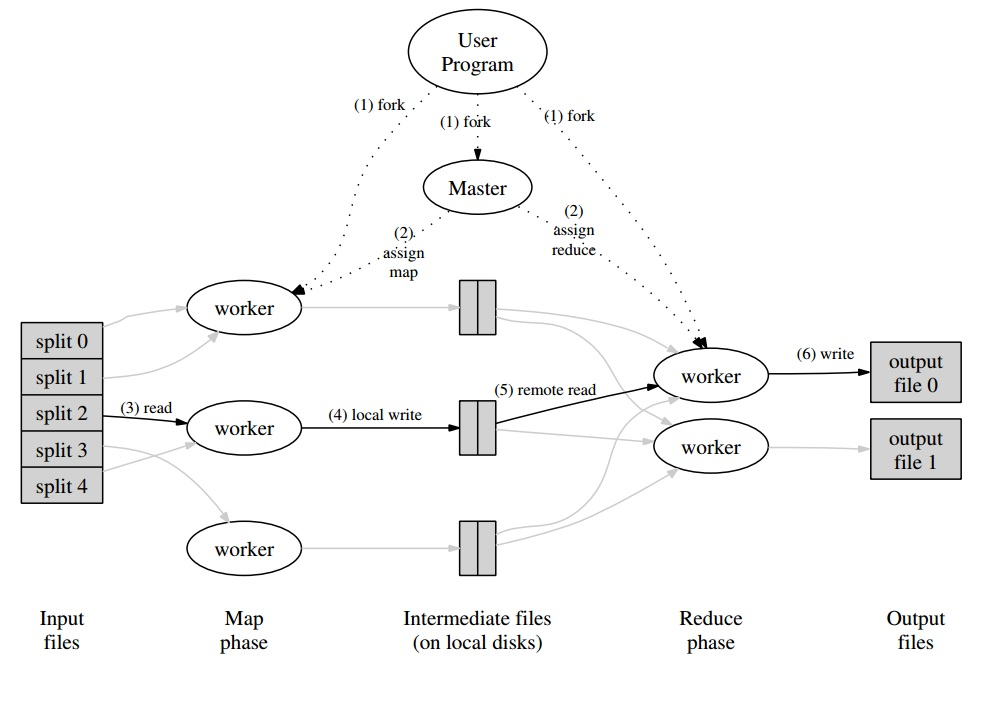
\includegraphics[width=1\textwidth]{mapreduce.jpg}
\caption{Map-Reduce architecture\cite{mapreduce}}
\label{fig:mapreduce}
\end{center}
\end{figure}

Traditional DBMS cannot cope with the scale and heterogeneity of the data sets
cited previously. Over time, models like MapReduce\cite{mapreduce}
Figure~\ref{fig:mapreduce}, Spark\cite{spark} and Storm appeared. Those
architectural models facilitated the parallelization of data analysis processes
at scale, running on commodity hardware. These systems are classified as batch
processing, meaning that all input should be collected into a batch before
processing it.

MapReduce and batch processing paradigms have been quite successful over the
years on large data-sets scenarios. But new needs are arising
and data analysts are becoming more demanding with their requirements. Batch
systems are designed to run with bounded data, imposing big latencies. In some
situations it is not feasible to wait hours to get back results from analytics.
One example could be monitoring microservices architectures where anomalies must
be investigated and fixed as soon as possible to avoid service disruptions.

\bigskip

To avoid latencies imposed by batch systems, hybrid systems were designed. One
paradigmatic example is Lambda Architecture \cite{lambda}. It consists of
two data processing systems running in parallel. One of the systems, known as
streaming system, will provide approximate results in nearly real time. To
obtain more precise results, a classic batch systems run over the same data-set.
Soon, these systems showed many problems; running two processing pipelines in
parallel is translated into many operational issues as well as more costs
\cite{kappa}.

In general, batch processing systems don't perform well on stream data-sets.
Stream data-sets, as defined in \cite{streamissues}, can be characterized as follows:

\textit{
\begin{itemize}
\item The data elements in the stream arrive online.
\item The system has no control over the order in which data elements arrive to
  be processed, either within a data stream or across data streams.
\item Data streams are potentially unbounded in size.
\item Once an element from a data stream has been processed it is discarded or
  archived — it cannot be retrieved easily unless it is explicitly stored in
  memory, which typically is small relative to the size of the data streams
\end{itemize}
}

\bigskip

It is clear that batch systems were one of the enablers of big processing pipelines,
but new data processing platforms are needed. In particular, data processing platforms
that are able to deal with stream data.

To overcome the limitations imposed by batch systems on streaming data, a few
alternatives appeared. Google developed MillWheel\cite{millwheel} and Google
DataFlow\cite{dataflow}. Those systems were designed with the previously exposed
problems in mind. The main differentiator was how unordered data was treated. To
facilitate working with unordered events, the next concepts were introduced\cite{dataflow}:
\textit{
  \begin{itemize}
  \item Windowing: slicing data into finite chunks for processing.
  \item Triggering: stimulating the output of a specific window at a grouping operation.
  \end{itemize}
}

This project will be focused on developing a data processing system using the
same principles that Google Dataflow and MillWheel are based on. 

\chapter{Objectives}
\label{chap:objectives}

\drop{I}{n} this chapter, the global objectives that have motivated the project
are described. As well as the more specific goals that want to be achieved.

\section{General Objectives}

The purpose of this project is to develop a distributed, fault-tolerant and
elastic streaming processing framework aimed for unbounded datasets. Given a
user defined topology of computations, the system will place them into a cluster
of nodes optimizing the resource utilization. Alcaudon abstracts away all the
difficulties involved in programming in a distributed environment. The user just
needs to define the computations, using the Alcaudon computation Interface, data
dependencies, and the system will take care of the execution. The system should be
easily deployed into cloud platforms such as Amazon Web Services, so it can cope
with bursts of load dynamically.

\section{Specific objectives}

Given the previous general description, objectives can be categorized into the
following sub-objectives.

\subsection{Provide an abstraction to create distributed computations}
One of the primary goals of this project is to provide abstractions to create
distributed streaming programs without distributed systems expertise. To achieve
this, Alcaudon should provide a computation API that allows clients to write
their business logic without knowing any details of the underlying
infrastructure.
Alcaudon should provide means to work with persistent state in user code. A
State API is provided to work with key-value pairs.

\subsection{Develop mechanisms to ensure exactly-once processing of records}

One of the biggest problems in distributed systems is to guarantee that a record
has been delivered and processed. The system will ensure that messages are
delivered exactly-once, without any change in user code.

To achieve exactly-once delivery in a performant manner, i.e., without two-phase
commits (citation needed), Alcaudon will enforce idempotency using probabilistic
data structures and state journaling.

\subsection{Provide tools to work with out-of-order data}

Unordered data is a reality in distributed environments. Some systems enforce
monotonicity of event time using the injection time instead of the event
generation time. Alcaudon will provide tools to work with non monotonic event
times.

\subsection{Implement a cluster scheduler}

Users of Alcaudon provide a directed acyclic graph of computations, and those
tasks should be placed into the cluster available resources. Cluster scheduling
usually leads to an NP-hard problem. The system will implement a scheduler based
on heuristics to set the tasks into the computing nodes.


\subsection{Allow extensibility of sources and sinks}
Some implementations for unbounded data sources, like socket, scala collections
and twitter will be available. But users will be able to extend Alcaudon to add
custom Sources and Sinks.

\subsection{Design and implement an elastic, fault-tolerant and scalable distributed architecture}
The system should have the properties described in the reactive manifesto(citation needed):

\begin{itemize}
  \item The system should be \textit{resilient}, meaning that in the face of a failure it should keep running.
  \item The system should be \textit{elastic}, in the face of an increase of load it
    should be responsive allowing adding new resources to cope with the new
    requirements.
\end{itemize}

It should make easy to add new nodes to the cluster, so the resources available
can change depending on the needs. This design towards a more cloud could make
easy to offer Alcaudon as a service.

\subsection{Provide tools for observability}

Since Alcaudon is a distributed system, debugging that kind of applications is
hard. Providing metrics on the state of the cluster as well as centralized logging
is mandatory.

\chapter{State of the art}
\label{chap:stateoftheart}

\drop{T}{his} chapter aims to explain the concepts and techniques in which
Alcaudon is based on. As shown in Figure ~\ref{fig:mindmap}. the project has foundations in
distributed systems, job scheduling, library design and data processing. In the
next subsections, those concepts will be analyzed in more depth.

\begin{figure}[!h]
\begin{center}
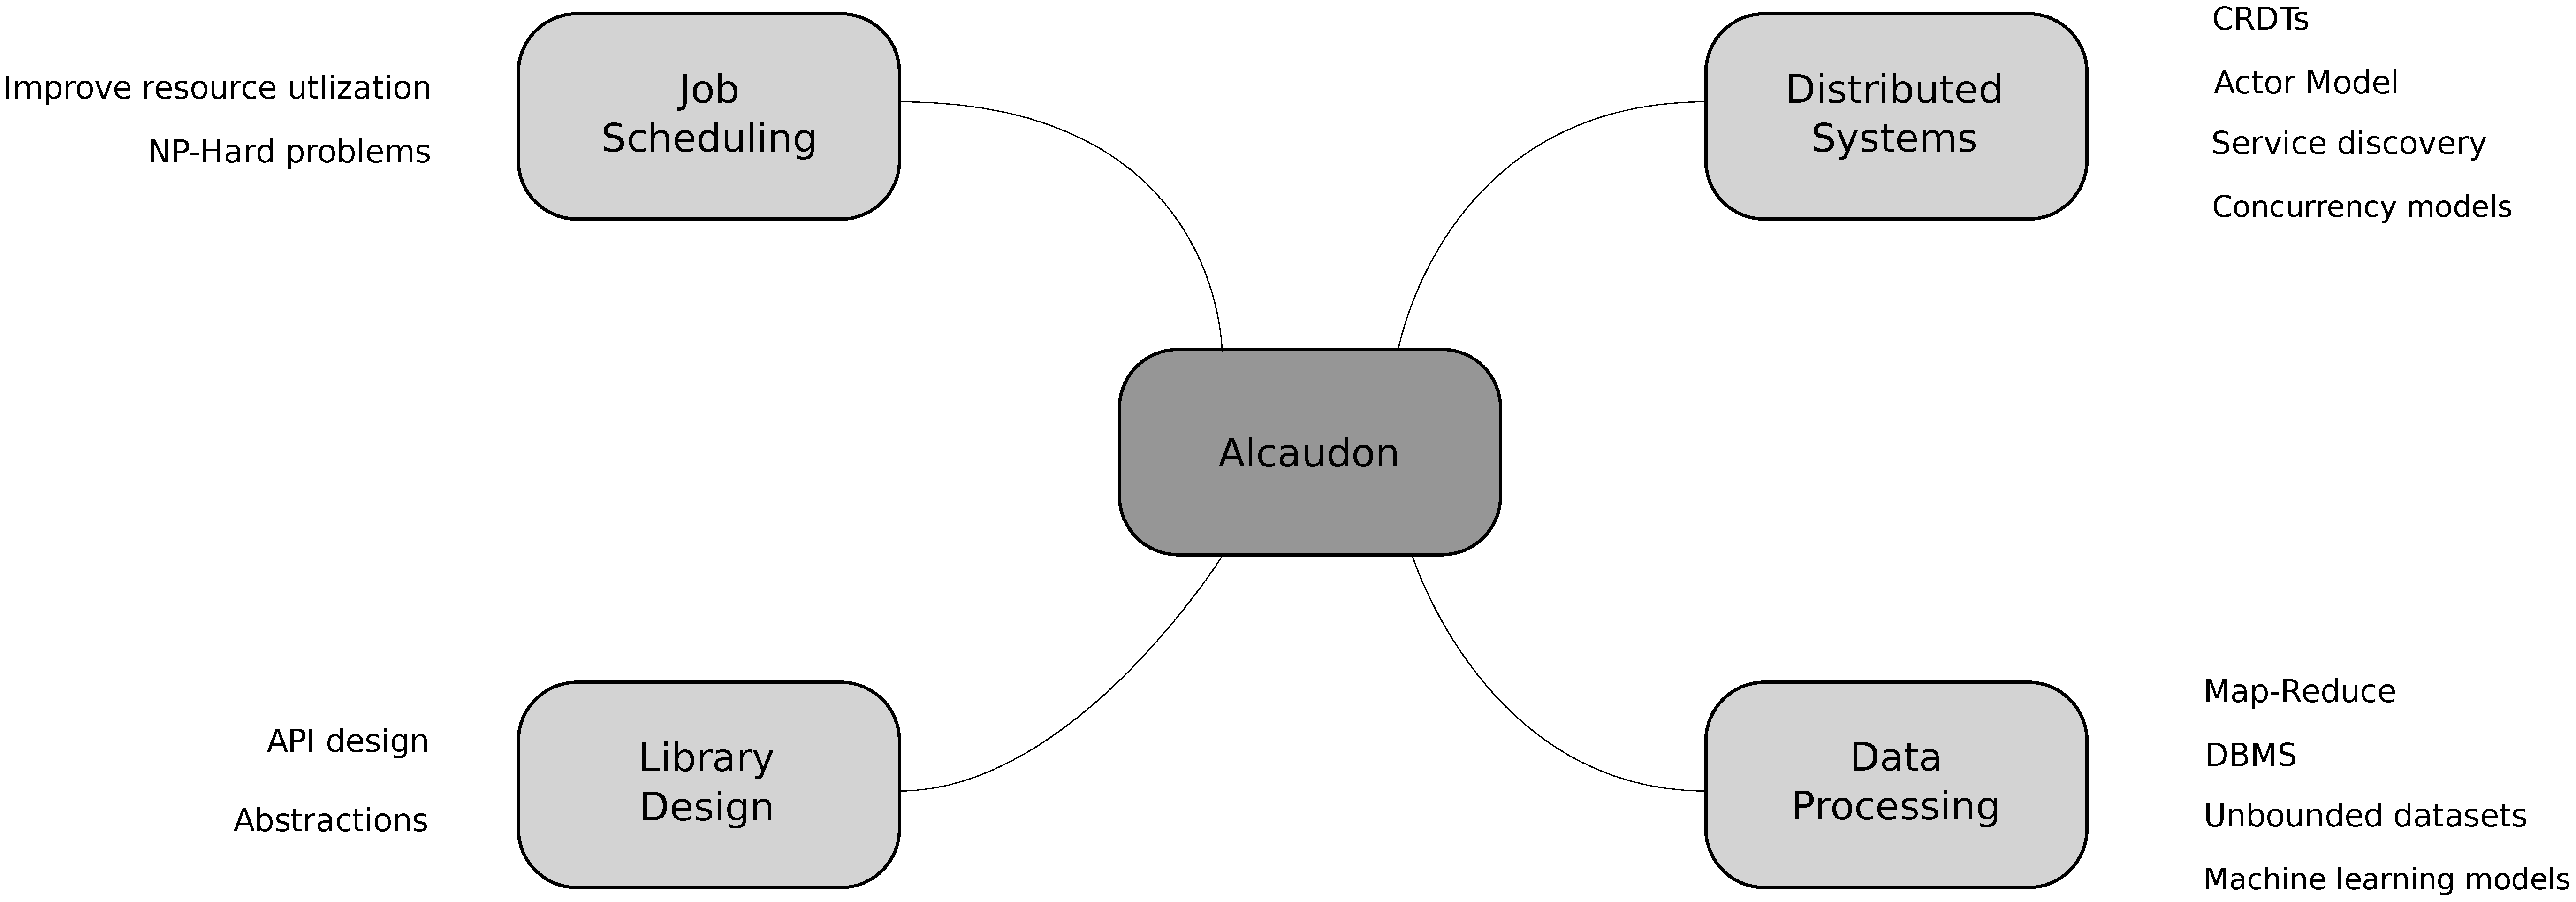
\includegraphics[width=1\textwidth]{mindmap.pdf}
\caption{Alcaudon foundations}
\label{fig:mindmap}
\end{center}
\end{figure}

\subsection{Data Processing}

According to a recent study by Cisco \cite{ciscosurvey}~\ref{fig:ciscodata} the
data storage is growing by 40\% yearly. This implies that that by 2020
datacenters will store over 1000 ExaBytes of information. Keeping that data in
silos without performing any use of it is a poor investment.

\begin{figure}[!h]
\begin{center}
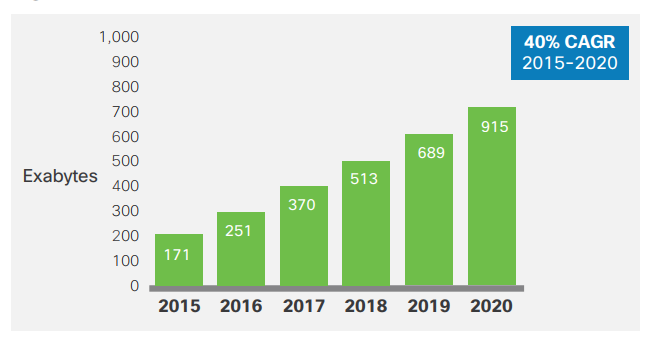
\includegraphics[width=0.8\textwidth]{ciscodata.png}
\caption{Actual Data Stored in Data Centers\cite{ciscosurvey}}
\label{fig:ciscodata}
\end{center}
\end{figure}

Processing those amounts of data using traditionals RDBMS is not practical, as they
are not designed to work with that much data. In the last years there have been
many ongoing efforts on providing tools to process and analyze large volumes of
data. Some examples could be MapReduce\cite{mapreduce}, Spark\cite{spark} and
many others. Before those frameworks appeared, there were some systems capable
of processing large amounts of data, like the supercomputers or HPC. One of the
main drawbacks of HPC is accessibility to those high end computers. Acquiring a
new Supercomputer in the event of a peak on data production is not feasible. For
companies, making an investment in a super computer is a big risk that in some
cases will not be reverted as profit. Another interesting point to make is that
Supercomputers perform well many floating-point operations per second. However,
in general, the computations executed in systems like MapReduce are simple
strings manipulation, counting and so on. Given these usage patterns, it seems
that supercomputers are more suited to perform scientific analysis.

Once the limitations of HPC for \textit{big data} scenarios have been described
it is possible to explore how modern internet companies are using computing
resources to process data. For new organizations, it is more sensible to take
advantage of commodity hardware to process large amounts of data. One of the
reasons is that there are many tools to distribute data processing among large
clusters of commodity machines. Once that job is done, those machines can be
turned off or used for other purposes. Working with those systems provides
flexibility, both in resource usage and innovation capacity. 

Even though systems such as Map-Reduce have been quite useful to process large
amounts of data, they start to have limitations in certain aspects. Currently,
the need of low latency in data processing is getting mandatory. Organizations
need to get insights about their data as soon as possible, in order to react
quickly to new trends. The systems described previously are classified as batch
systems, as they are oriented to process historical datasets and not
\textit{real time data}. There have been some adaptations to these systems, using
approaches like micro-batching where data is processed in smaller batches,
however the latency is still big. These new needs for data processing have lead
to the design and development of systems specialized in unbounded data
processing. These systems try to reduce the time between the event generation
and its processing. Alcaudon fits in this category of data processing systems,
as one of its aims is being able to process unbounded data sets with low
latency.

\subsubsection{Cloud Computing}

Cloud computing might be seen as a recent development. However, during the 1990s
researchers at Xerox PARC started to develop ideas around what they named
\textit{ubiquitous computing}. The idea was to have computing devices
interconnected and exchanging data about almost everything. This idea was ahead
of his time because there were just a few networks around. And devices such as
cameras and microphones were still quite big, etc. Even though if this definition is
translated to 2017 seems to fit quite perfectly on how devices behave nowadays.
Cars, fridges, watches, smartphones and anything that can have a network
interface is connected to the internet. Huge amounts of data are being published
and stored into the what is now known as \textit{the cloud}. There is not a
clear definition for what \textit{cloud computing} is. For the purposes of this
text, cloud computing could be defined as a pool of shared computing and storage
resources that can be provisioned and released on demand. Given the huge amounts
of data that users store into the \textit{cloud}, companies need to outsource
computing and storing capacity, since building datacenters is a huge investment.
In the last decade, computing infrastructure offering has changed radically.
Companies such as Amazon Web Services are able to offer servers, storage and
services on demand at scale, from 1 server to 1 million servers. Having the
ability to start and stop servers on demand has democratized the ability to
process large amounts of data for many organizations. For example, a startup can
kickoff with just one server to process data. Once the business starts growing,
it can take advantage of the elasticity provided by cloud computing services,
and start using more servers to cope with the load. This is one of the reasons why
data processing systems should be designed to scale out as there are more
computing needs.
Alcaudon, as an elastic data processing system, will be able to adapt to
different loads as the computing needs increase.. It will be able to use more
computing resources dynamically as more servers are added to the pool.

\subsection{Distributed systems}
\label{subsection:distsys}

Distributed systems can be defined as a set of computer programs, executing on
one or more computers, and coordinating actions by exchanging \textit{messages}
\cite{GuideReliable}. Those computers are usually located in a \textit{computer
  network}, a collection of computers interconnected by hardware that supports
message passing and implement routing protocols. But if this definition is taken
to the extreme, a modern multi-core processor can be characterized as a
distributed system, with many components exchanging information in a network and
coordinating actions to get work done. To some extent, it is possible to see
distributed systems as a super set of concurrent systems.

A more common example of a distributed system is a user requesting a web page to
a server with his smartphone. This example is a typical \textit{client-server}
model. This \textit{simple} action involves the interaction of various services
such as DNS servers, load balancers, HTTP proxies and HTTP servers. All these
services use a network as a mean to interchange messages as shown in figure
~\ref{fig:client-server}.

\begin{figure}[!h]
\begin{center}
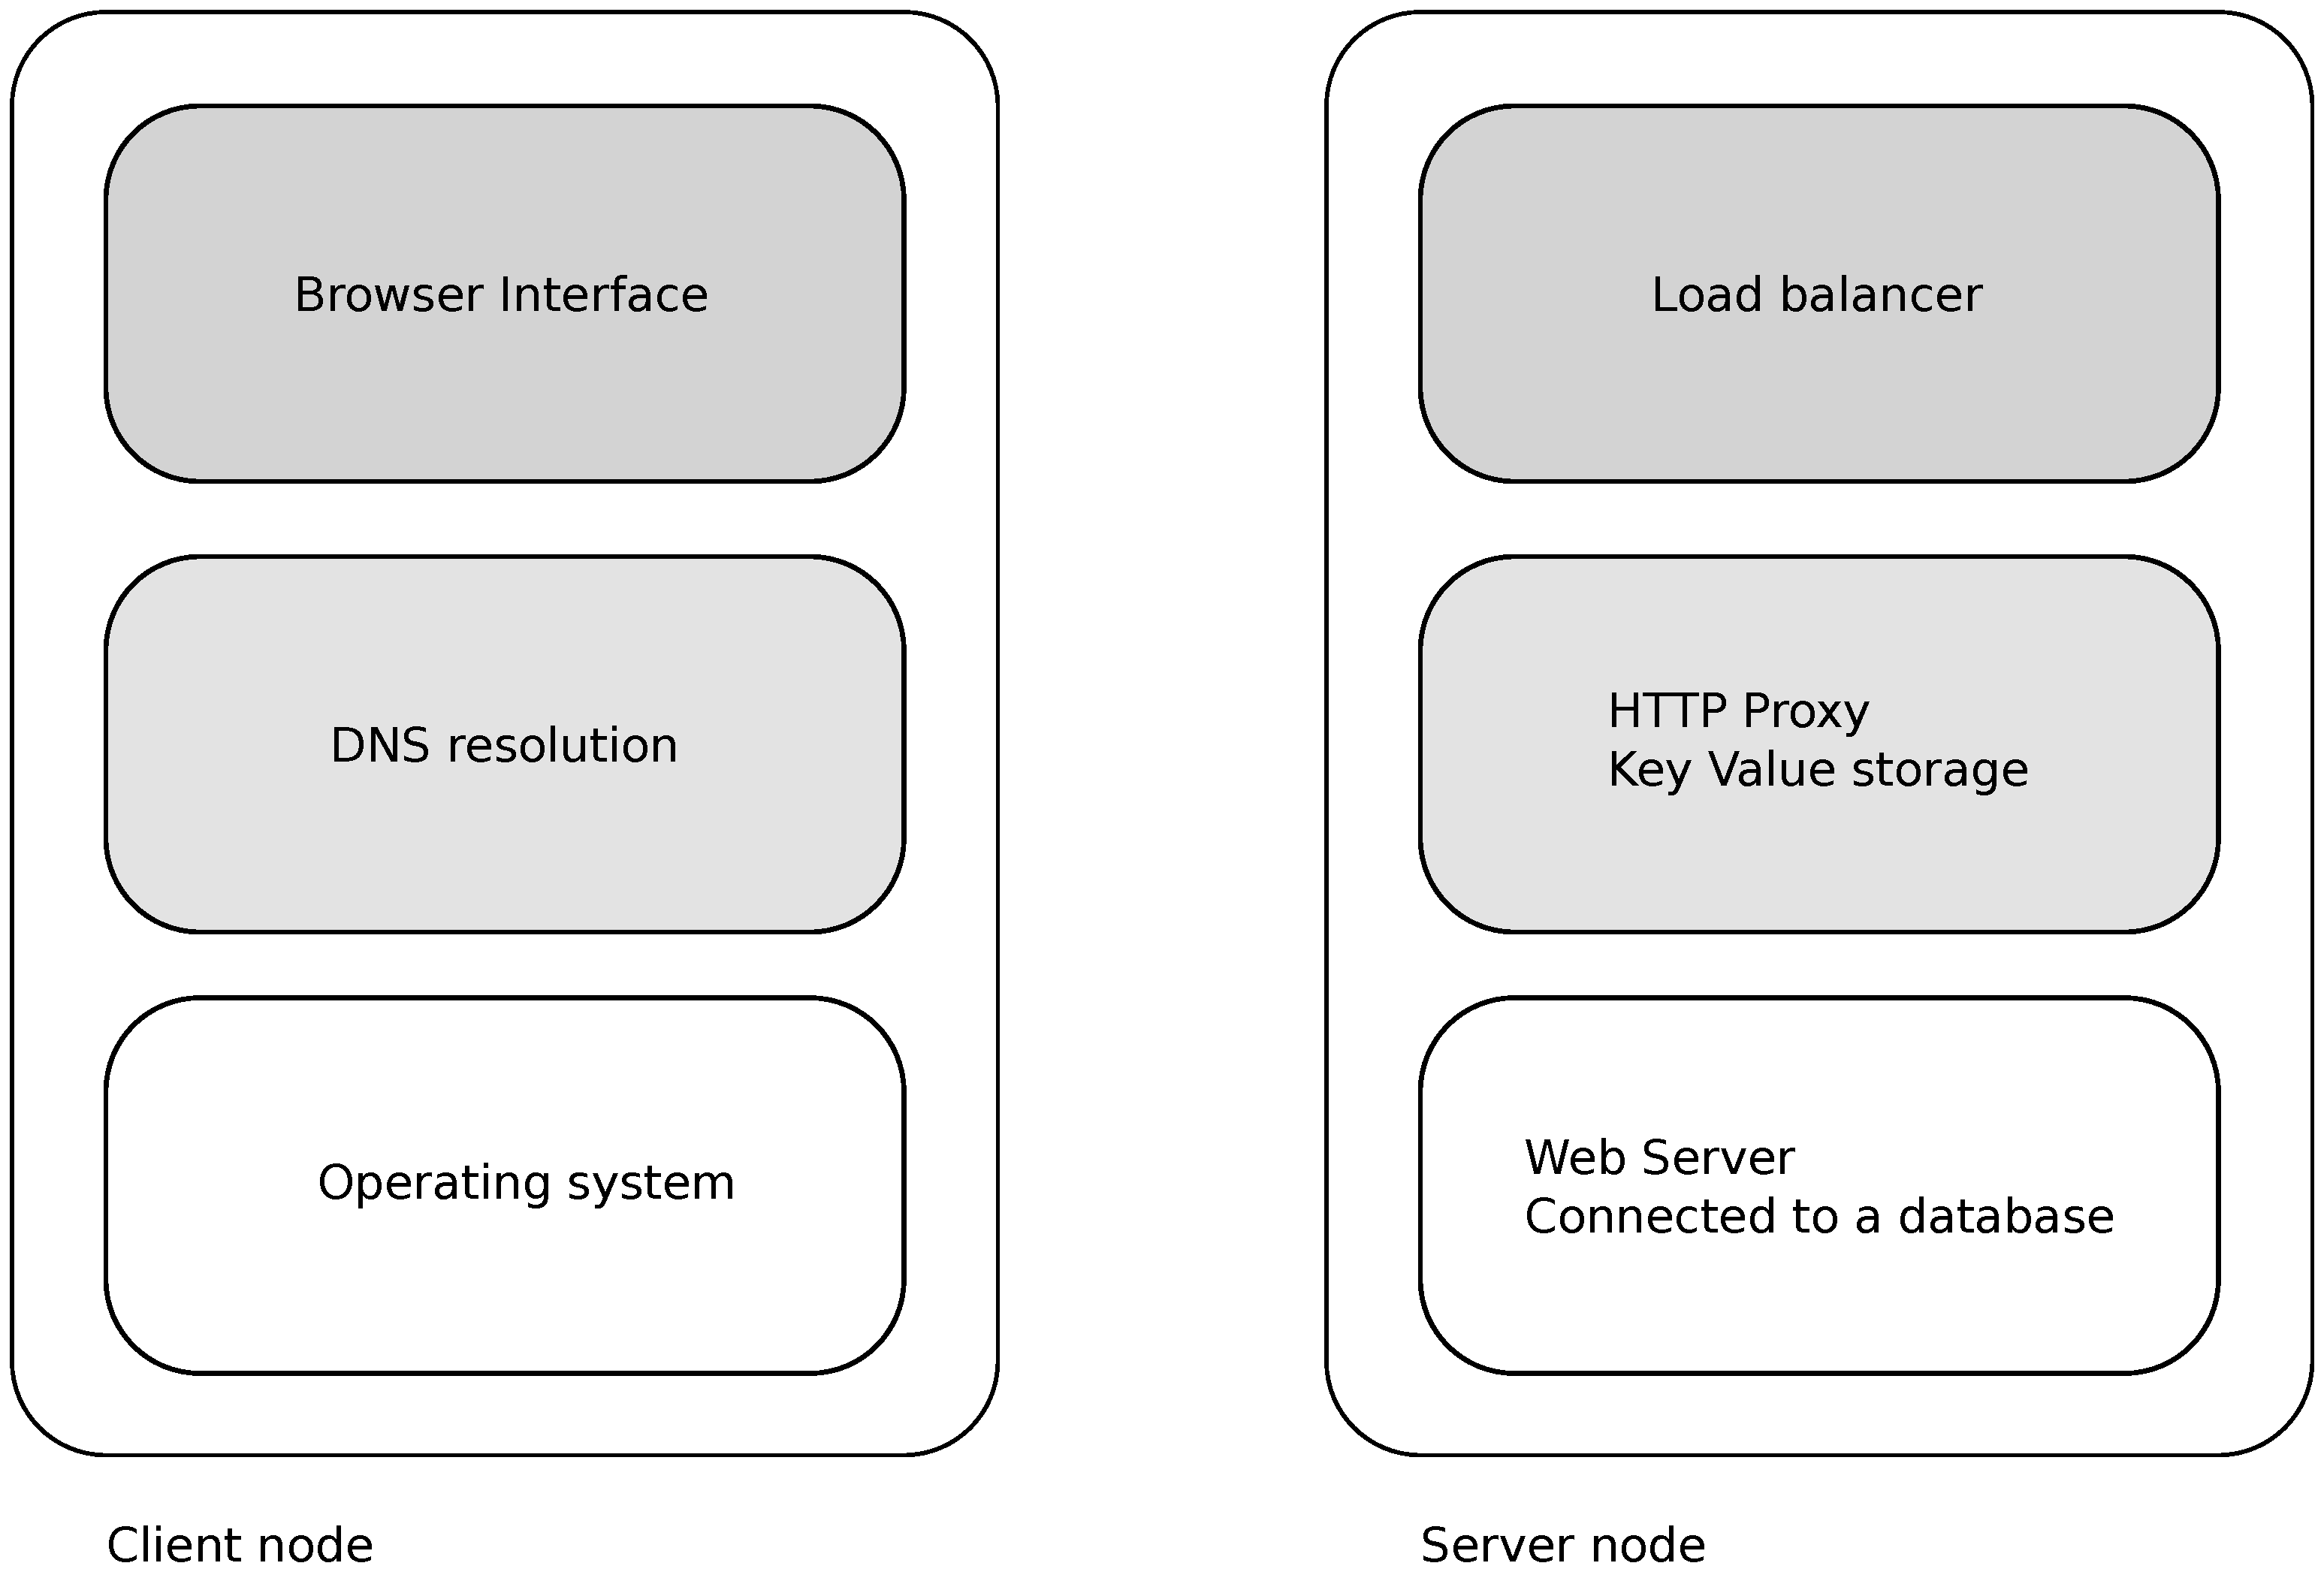
\includegraphics[width=0.7\textwidth]{client-server.pdf}
\caption{Client-server architecture}
\label{fig:client-server}
\end{center}
\end{figure}

As it has been previously discussed, distributed systems are very common
nowadays. They are present in fields like database systems, internet of things,
data processing and many more.

There are some reasons that make more convenient to work with distributed
systems, but the main reason is ability to scale. As defined in \cite{cloudadmin}
\begin{quote}
  A system's ability to scale is its ability to process a growing workload,
  usually measured in transactions per second, amount of data or number of
  users.
\end{quote}

Distributed programming can help designing systems with the ability to scale given
the following properties:

\begin{figure}[!h]
\begin{center}
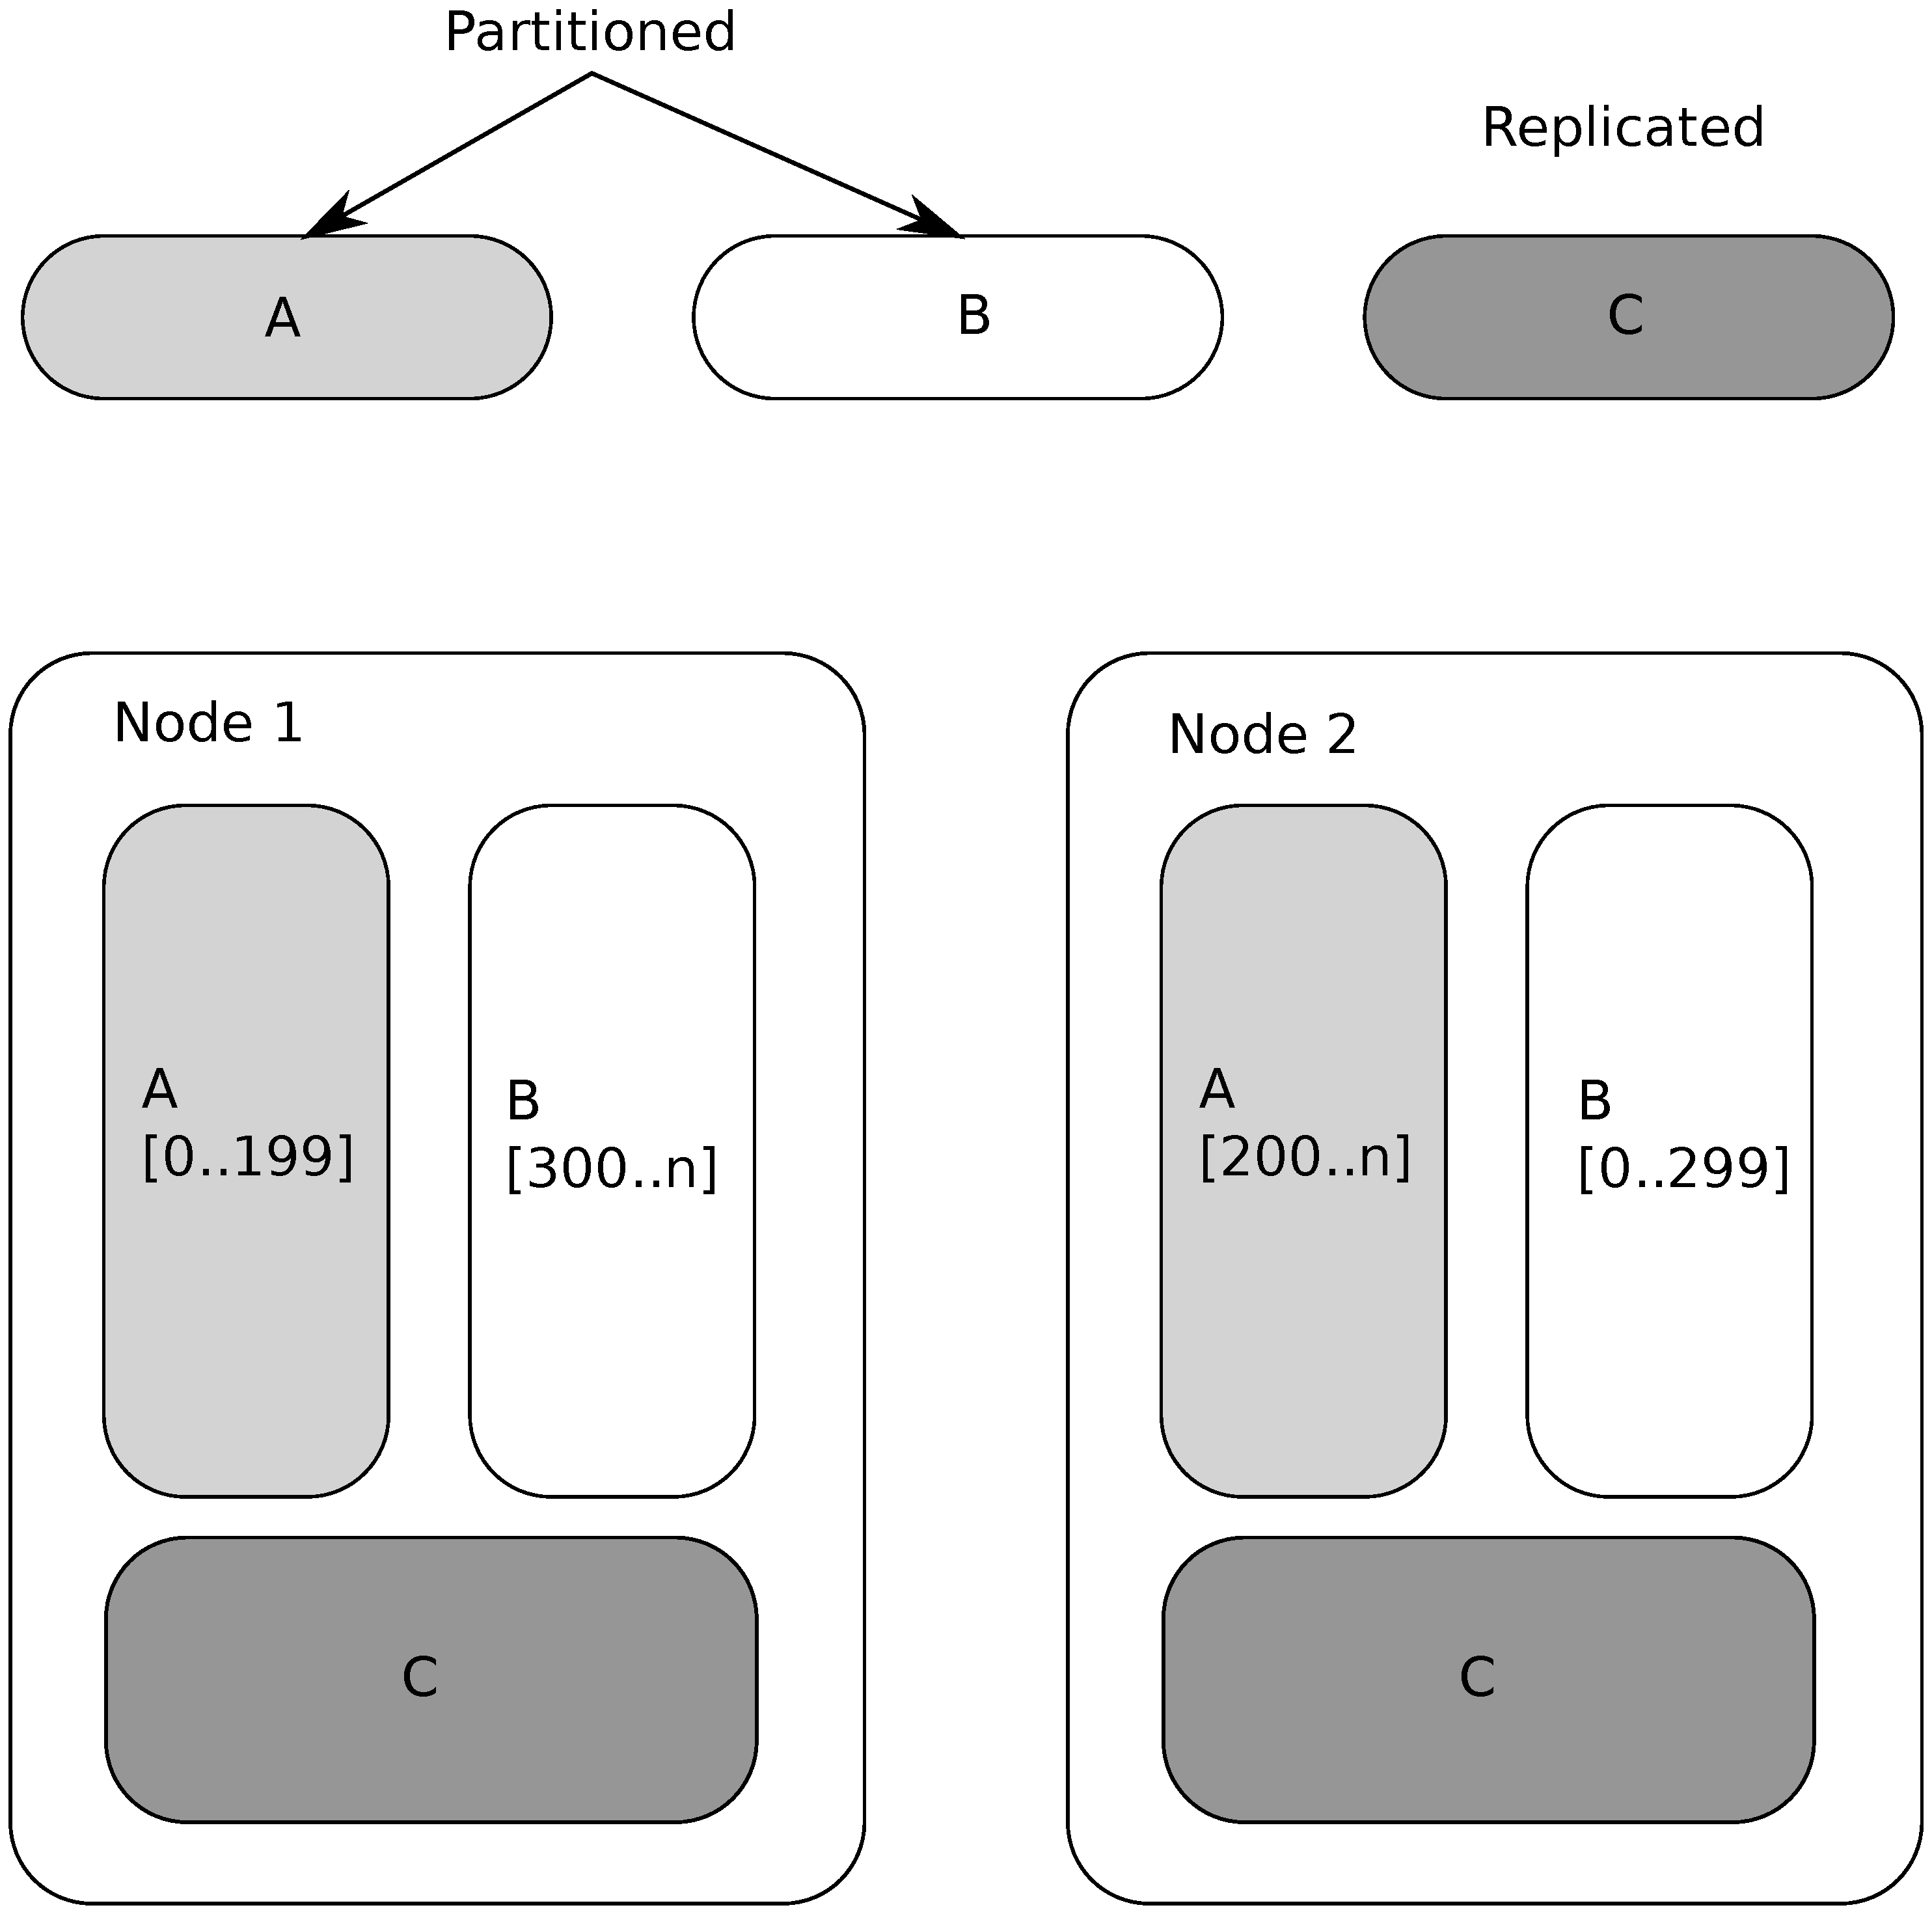
\includegraphics[width=0.7\textwidth]{partition-rep.pdf}
\caption{Partitioning and Replication}
\label{fig:partitioning}
\end{center}
\end{figure}

\begin{itemize}
\item \textit{Reliability}: Achieved by \textit{replication} and/or
  \textit{partitioning} as illustrated in Figure ~\ref{fig:partitioning}.
\item \textit{Elasticity}: Since the systems are designed to work in
  coordination with other processes, it is possible to add more resources to
  handle increasing workloads. But there is an upper limit imposed by the
  coordination model used.
\item \textit{Parallelism}: This is a natural outcome of having multiple resources, they
  can get work done in parallel.
\item \textit{Price/performance ratio}: Scaling vertically (using more powerful
  compute nodes), has upper limits both in available technology and in costs. As
  shown in Figure ~\ref{fig:highend} the performance gap between a high end
  server and a cluster of commodity hardware nodes is tolerable. Another factor
  to take into account when distributed systems are used is the cost of
  networking communications, as it implies an overhead in the computations.
\end{itemize}

\begin{figure}[!h]
\begin{center}
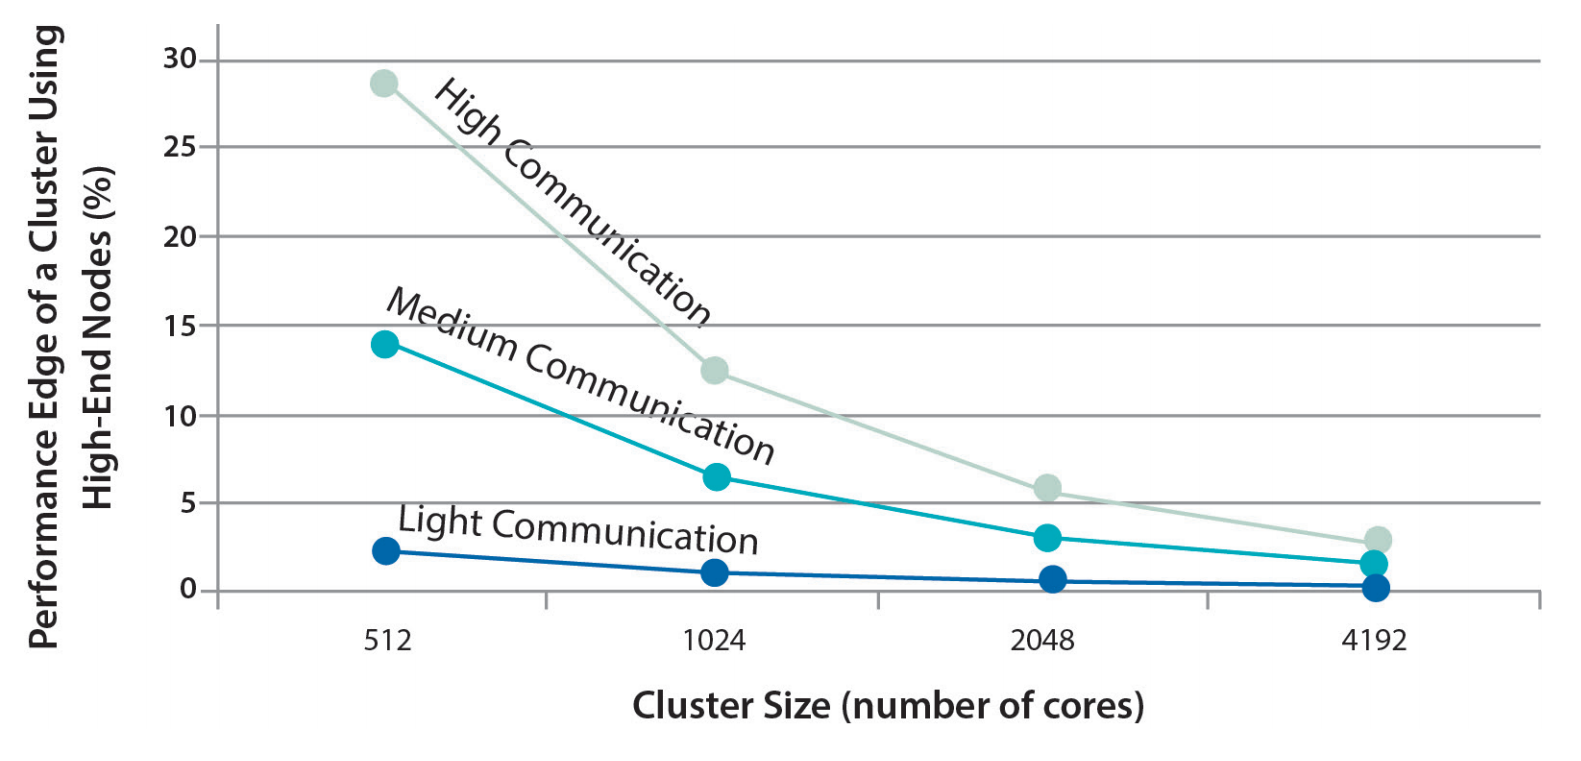
\includegraphics[width=1\textwidth]{scalingcost.png}
\caption{Performance advantage of a cluster built with large SMP server nodes
  (128-core SMP) over a cluster with the same number of processor cores built
  with low-end server nodes (four-core SMP), for clusters of varying
  size.\cite{Datacenter}}
\label{fig:highend}
\end{center}
\end{figure}

\subsubsection{Taxonomy of a distributed system}

Once described what distributed systems are and why they are useful, it is
possible to define a taxonomy of distributed systems topics such as coordination
algorithms, global state collection, distributed consensus, etc.

As it can be seen the topic is wide, so for this documents only
\textit{distributed snapshots}, \textit{membership protocols} and \textit{time
  in distributed systems} will be covered.

\begin{itemize}
\item \textit{Time in distributed systems}:
  Programmers are used to think in sequential programs, where computation steps
  are executed one after the other. The reality in distributed and concurrent
  systems is quite different. Knowledge about global state among all the nodes
  in the system is likely to be outdated. A naive solution to this problem is
  using synchronization based on wall clocks. However, the notion of
  synchronized clocks among nodes is impractical. Protocols like NTP\cite{ntp}
  can have skews up to 1000 seconds, an unacceptable time in some cases. Google
  makes heavy use of hardware-assisted time synchronization using GPS clocks and
  atomic clocks to ensure global consistency for their database
  Spanner\cite{180268} that can drift up to 100ms. Given the exposed facts, the
  only assumption that can be taken about global state that is partially
  ordered. A formal definition for partial order is \cite{book:lattices}:
\begin{definition}{Partial order}
  Let $P$ be a set. An order (or partial order) on $P$ is a binary relation
  $\leq$ on $P$ such that, for all $x$, $y$, $z \in P$,
  \begin{enumerate}
  \item $x \leq x$
  \item $x \leq y$ and $y \leq x$ imply $y$
  \item $x \leq y$ and $y \leq z$ imply $x \leq z$
  \end{enumerate}
\end{definition}
  Given the exposed facts, message order in distributed systems is partial. In
  environments where the message flow is unbounded the notion of completeness is
  weak. There is no guarantee about when all the messages up to a moment $T_n$
  have been received or processed. To deal with this, Alcaudon uses watermark
  heuristics. A watermark heuristic defines that up to the instant $T_i$ there
  are high chances that all messages up to that point have been received.
\item \textit{Distributed snapshots}:
  Since Alcaudon aims to be a fault-tolerant system, guarantees about persistent
  state must be enforced. To design a resilient system, persistent state
  snapshots should be taken. There are distributed algorithms to deal with this
  problem such as Lamport, bla, bla . In general, those algorithms are focused
  on taking a global state snapshot that given the constraints presented in the
  previous section is a hard problem to solve. In Alcaudon this obstacle is
  solved by taking snapshots by computation. There is no need of a global
  snapshot since persistent state is local to each computation.

\item \textit{Membership protocols}: Another crucial aspect on an elastic
  distributed system is how to handle cluster membership. It is possible to
  classify them into two categories: static membership and dynamic membership.
  Static membership has a fixed list of cluster members that do not change along
  the life of the cluster. With this static membership there is a chance that at
  some point in time, some members of the cluster will not be available. Since
  cluster membership image is static, thew will be seen as accessible. The other
  approach is to use dynamic membership. It consists on having initial knowledge
  about a subset of the available nodes and later on, via gossiping
  protocols\cite{gossip} new nodes can \textit{join} the cluster. This mechanism
  is also able to handle when nodes become \textit{unavailable}. For Alcaudon
  the latter membership category is more suitable. Since one of the goals is to
  provide elasticity, in this case the system will be able to be scaled in the
  need of more computing power.
\end{itemize}

\subsubsection{CRDT}

As previously presented, Alcaudon will be founded watermark heuristics. In order
to implement these heuristics, there is a need for some global knowledge about
latest processed events to keep track of the progress of ingested events into
the system. Each computation should be able to have partial knowledge of the
last watermark, and that depends on the state of a its dependencies. One of the
goals of the system is to avoid centralized coordination as much as possible, so
consensus based stores are discarded. One available option is Convergent
Replicated Data Types (CRDT)\cite{crdt}.


\begin{definition}{Merge properties}
  Let $P$ be a set. An order (or partial order) on $P$ is a binary relation
  $\leq$ on $P$ such that, for all $x$, $y$, $z \in P$,
  \begin{enumerate}
  \item $x \leq x$
  \item $x \leq y$ and $y \leq x$ imply $y$
  \item $x \leq y$ and $y \leq z$ imply $x \leq z$
  \end{enumerate}
\end{definition}

TODO


\subsubsection{Distributed system reliability}

Building distributed systems is not an easy task. In this subsection, different
failure scenarios that can happen in a distributed environment will be presented.

As proposed by \cite{GuideReliable}, it is possible to classify system error
causes as follows:
\begin{itemize}
\item \textit{Hardware failures}: These kind of failures are inevitable, since
  hardware has a life cycle and some components might fail or maintenance for
  components should be taken care of.
\item \textit{Software failures}: Software is becoming more and more complex.
  Software complexity errors such as coding errors, misguided software design,
  memory leaks or inadequate specifications are inevitable. There are countless
  examples of millionare losses, like when in 1999 NASA lost a Mars orbiter
  spacecraft because one team was working with Imperial units while another used
  metric units.
\item \textit{Complexity}: Developing software in distributed systems is
  complex. The notion of global state or order is fuzzy. Asynchronous
  communication is the norm. Regular developers are used to sequential
  computations, and getting familiarized to work within this environment is hard
  and can lead to bogus implementations. Luckily the use of formal verification
  is growing in the field, using tools such as TLA+\cite{tla} by Lamport. The
  usage of these techniques helps to tackle the inherent complexity with strong
  foundations.
\item \textit{Lack of failure detectors}: Most distributed systems try to detect
  failure just by using timeouts. This measure is quite straightforward to
  implement and reason about. The main drawback is that these techniques are
  raw. Vogels \cite{vogels} proposes a refinement over plain timeouts for
  failure detection, using more meta-information about the environment where
  the distributed system is running; reasoning about operating system metrics,
  networking metrics and disseminated probes, failure detection can improve.
\item \textit{Hostile environments}: There has been enumerated some reliability
  threats, which distributed systems need to deal with. Those threats are in
  \textit{control}, meaning that the developers of the system should anticipate
  them. Designing the systems so they are ready to deal with the exposed
  problems. However those systems run in shared networks where security threats
  are a reality. It is a wide field and it is becoming more and more important
  to take all the possible measures to avoid security vulnerabilities.
\end{itemize}

As a final note about other problems, there are costs associated with
distributed programming; network latency, fault-tolerance mechanisms and
consensus can have impact in the throughput achieved by a system. In
\cite{189908} a metric named Configuration that Outperforms a Single Thread
(COST), is proposed. It measures the number of cores needed to outperform a
single threaded implementation. In these experiments, there are many distributed
processing frameworks that don't perform properly when compared to single node
implementations. As a conclusion, there are scenarios where the costs associated
with distributed computing are higher than the gains.

Alcaudon's goal is to provide users a simple but powerful interface that enables
them to parallelize and distribute computations for unbounded datasets without all
the described problems.

\subsubsection{Actor Model}

To tackle all the complexity described in previous sections there is a
computation model that is well suited: the actor model.

The actor model provides a high level abstraction to deal with concurrent and
distributed systems. The theoretical model was developed by Carl Hewitt in
the seventies, but it was popularized by Erlang programming language\cite{erlang}
developed by Ericsson.

It can be characterized as follows:
\begin{itemize}
\item Actors communicate via asynchronous messages
\item Actors manage their state
\item In the event of a message response they can:
  \begin{itemize}
  \item Create new child actors
  \item Send messages to another actors
  \item Stop actors (even themselves)
  \item Change their behavior for the next messages
  \end{itemize}
\end{itemize}

Since distributed systems communicate asynchronously, this model fits perfectly,
because, even in single node environments, all the computations are executed in
response to asynchronous messages. The fact that the shared state among actors
is minimal helps to tackle all the inherent complexities around concurrency.
Another interesting outcome from designing the systems using message passing is
that creating protocols comes naturally in this model. The ability to change
their behavior depending on the incoming messages makes easy to model finite
state machines that fit perfectly with protocol design.

There are many implementations available\cite{wikiactor}, but the more popular
and stable versions are the Erlang programming language and Akka. Both versions
have similar features, in fact, Akka is highly inspired by Erlang. Nevertheless
Akka is built on top of the JVM, making it the most interesting implementation
available due to the vast ecosystem accessible around the JVM.

Akka has some extensions to the actor model that make it quite interesting to
build distributed systems.
\begin{itemize}
\item Actor supervision: One interesting approach of actor based design is how
  to handle failures. Each actor has a supervisor that handles its life-cycle,
  exceptions included. With this supervision schema it is easier to isolate failure
  scenarios into concrete actors instead of affecting the whole system. Each
  supervisor can define a strategy to apply when a child actor fails, i.e.
  restarting the actor or stopping it. This is highly beneficial because error
  handling logic is separated from business logic. These patterns resemble how
  ships are built, where the hull is compartmentalized into different watertight
  bulkheads. Therefore, if the hull is broken, the failure is limited to that
  bulkhead without compromising the ship stability. Alcaudon will benefit from
  this pattern to achieve fault-tolerant computations. One actor supervision
  tree can be found in figure~\ref{fig:supervision}.
\item Logical addresses: Each actor has a virtual address based on the actor
  system and its hierarchy. This helps providing location transparency, as
  actors can change their physical location and the framework will take care of
  routing messages to the new actor location.
\item Clustering: Support for distributed actors is provided, combined with
  logical addresses makes facilitates writing distributed applications.
\item Persistence: Akka supports actor state persistence. It is implemented as
  an append-only log. That technique is commonly used as transaction log in
  traditional databases, each change is appended to the transaction log. In case
  of a failure, those events are applied again to the in memory database
  buffers. To avoid long recovery times, snapshots from memory are taken
  regularly so the recovery process just needs to re-apply changes from that
  point. Akka persistence is implemented as described. This feature fits very
  well to mantain Alcaudon persistent state of computations, since computations
  can be defined as actors.
\end{itemize}

\begin{figure}[!h]
\begin{center}
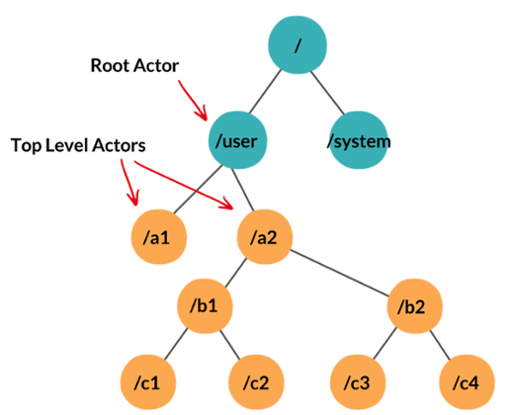
\includegraphics[width=0.8\textwidth]{supervision.png}
\caption{Actor supervision tree}
\label{fig:supervision}
\end{center}
\end{figure}

In conclusion, the actor model is a good computational model to base Alcaudon
on. It has properties that allows tackling all the presented difficulties around
writing distributed systems properly.

\subsection{Job scheduling}

Computations in distributed data processing clusters are expressed as a
dataflows. They can be considered as a direct acyclic graph (DAG) as the one in
Figure~\ref{fig:dataflow}.

\begin{figure}[h!]
\begin{center}
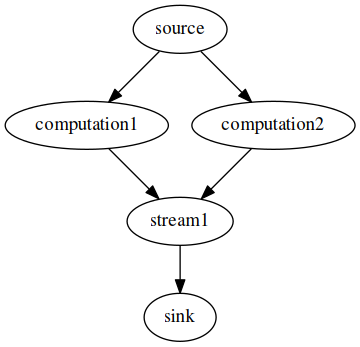
\includegraphics[width=0.6\textwidth]{dataflow.png}
\caption{Dataflow}
\label{fig:dataflow}
\end{center}
\end{figure}

One open problem in the construction of distributed data processing systems is
how to place those computations represented as a DAG, given a set of computing
nodes. This problem is known as the flexible Job-shop scheduling problem and it
has been widely studied during the last 60 years. One graphical example for $3$
jobs to be scheduled along $3$ machines can be seen in Figure~\ref{fig:jssp}.
As defined in\cite{jobshop2}:

\begin{definition}
In the flow shop scheduling problem we have a set of $n$ jobs that must be
processed on a given set of $m$ machines that are located in a fixed order. Each
job $j$ consists of a sequence of $m$ operations, where the $i$-th operation
must be processed during $p_{ij} \in \Z^{+}$ Time units without interruption on
the $i$-th machine. A feasible schedule is one in which each operation is
scheduled only after all operations preceding it in its job have been completed,
and each machine processes at most one operation at a time. A natural
generalization of the flow shop problem is to not require jobs to be processed
on all machines, i.e., a job still requests the machines in compliance with
their fixed order but may skip some of them. We will refer to this more general
version as generalized flow shops or flow shops with jumps. Generalized flow
shop (and thus flow shop) scheduling is a special case of the acyclic job shop
scheduling, which only requires that within each job all operations are
performed on different machines, which in turn is a special case of the general
job shop scheduling, where each job may have many operations on a single
machine. For any given schedule, let $C_j$ be the completion time of the last
operation of job $j$. We consider the natural and typically considered
objectives of minimizing the makespan, $C_{max} = max_j C_j$ , and the
\textit{sum of weighted completion times}, $\sum w_jC_j$ , where $w_j$ are
positive integers. The goal is to find a feasible schedule which minimizes the
considered objective function.
\end{definition}

\begin{figure}
\begin{center}
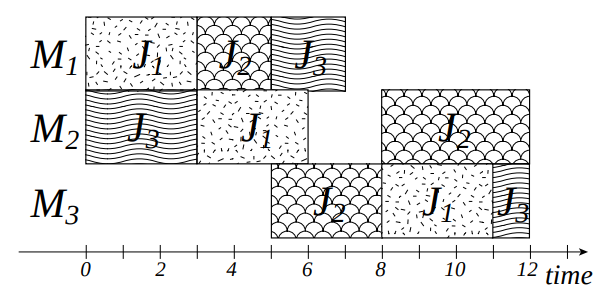
\includegraphics[width=0.6\textwidth]{jssp.png}
\caption{ A Gantt-Chart representation of a solution for a $3m \times 3j$ job scheduling problem\cite{geneticbook}}
\label{fig:jssp}
\end{center}
\end{figure}

Computing an optimal solution for this problem is a well known NP-hard
problem\cite{nphard}. Given this fact, all the proposed algorithms to solve this
problem are approximation algorithms. Some of the techniques used are listed
below:

\begin{itemize}
\item Algorithms based on priority rules and active schedule generation
\item \textit{Shifting bottleneck}
\item Simulated annealing
\item Tabu search
\item Genetic algorithms
\end{itemize}

How alcaudon solves this issue.

\subsection{Library design}

Humans have been using abstraction since the very beginnings of their existence.
The reality around is too complex to understand every detail of it. Thus,
abstraction is a really excellent tool to extract just the relevant facts about
the studied phenomenons. Computer Science, Software Engineering and Electrical
Engineering combine different abstractions in order to to build complex systems
in a manageable way.
Computer Science provides the tools whose roots are based on mathematical
foundations such as automaton theory, lambda calculus, language design, data
structures, etc.
Using those ideas, software engineering can be seen as the bridge between
hardware and computer science. It builds abstractions based on both worlds such
as operating systems, that hides the details of specific hardware and exposes an
uniform interface. And the list goes on. The main goal of abstractions is to
provide ways to reason about different problems with a limited scope.
As it has been exposed, providing tools that hide all the complexities is key to
build more complex systems. One of the main goals of the field since the late
60s has been to build reusable software\cite{reuse}. There have been many
advances in code reuse, from libraries and frameworks that are used to build
software on top them, to software as a service (SaaS). SaaS exposes public HTTP
API as the entry point to their functionality. This category of software reuse
can be the end of the spectrum, since the client just has knowledge about
the exposed interface and does not know anything about the underlying parts of the
system.

\begin{figure}[!h]
\begin{center}
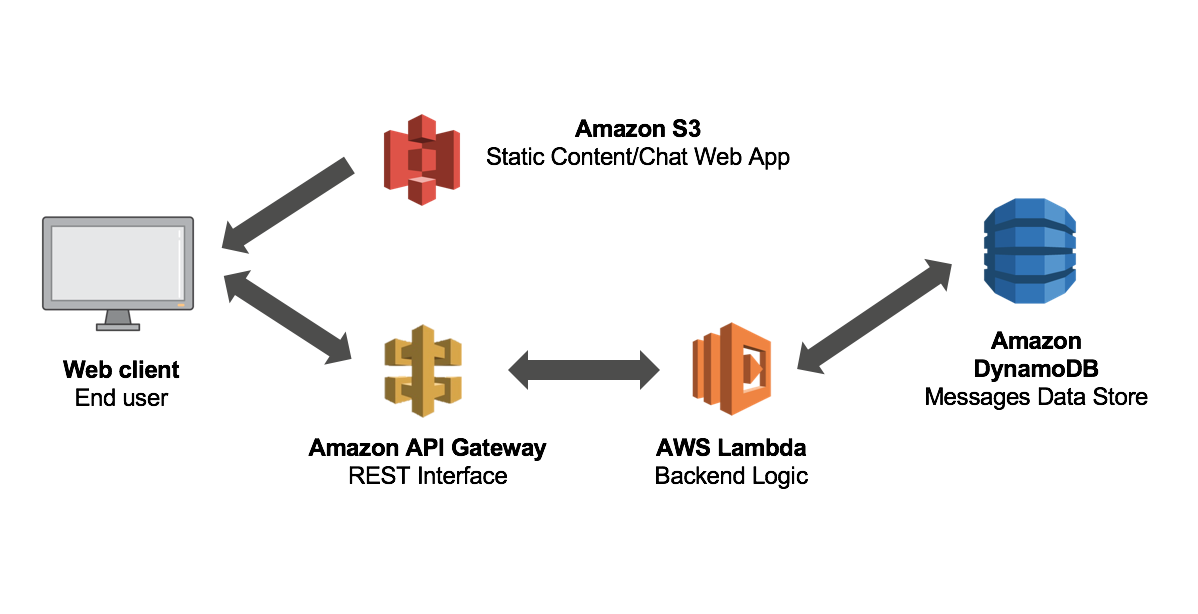
\includegraphics[width=0.8\textwidth]{serverless.png}
\caption{Serverless architecture example\cite{awsserverless}}
\label{fig:serverless}
\end{center}
\end{figure}

One recent trend in industry is serverless architecture like the one shown in
Figure~\ref{fig:serverless}. This programming model has foundations in reactive
programming, and it is based on providing code to produce computation results as
response to changes or events. In this paradigm it is just needed to provide
code implementing certain interface~\ref{code:lambdalisting} to handle events,
such as database changes, and the system will take care of deploy and run those
pieces together. As it can be observed, abstraction is going upwards and
programmers just need to take care of writing business logic and building
robust programs.

\begin{lstlisting}[language=java, frame=trBL, label=code:lambdalisting, float=ht, caption = {AWS Lambda Interface}]
  public interface RequestStreamHandler {
    public void handleRequest(InputStream inputStream, OutputStream outputStream, Context context)
    throws IOException
  }
\end{lstlisting}

Alcaudon philosophy is similar to the serverless architecture. The goal is to
provide abstractions around unbounded datasets so programmers just take care of
defining their computations and dependencies. Alcaudon will provide a simple
interface so the details to know about the system are minimized.

\chapter{Methodology}
The software methodology used to develop this project will be described in this
chapter. Agile methodologies have been used to drive Alcaudon's development.

Agile methodologies help organizing software development life cycle. They are
focused on iterative development and adaptability. The term was coined during
the early 2000s in the \textit{Agile Manifesto}\cite{manifesto}. The manifesto
has this set of principles:

\begin{itemize}
\item Individuals and interactions over processes and tools
\item Working software over comprehensive documentation
\item Customer collaboration over contract negotiation
\item Responding to change over following a plan
\end{itemize}


\begin{figure}
  \centering
  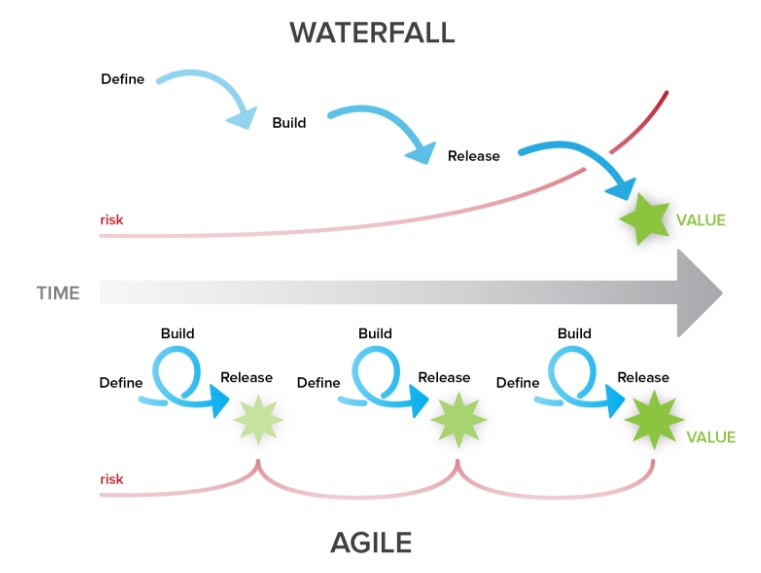
\includegraphics[width=0.8\textwidth]{agile.jpg}
  \caption{Waterfall vs Agile Methodologies\cite{waterfall}}
  \label{fig:waterfall}
\end{figure}

The main goal of these methodologies is to improve communications between all
the stakeholders in a project. This focus on continuous communications reduces
risks and provides value since the very beginning of the project. One of the
outcomes of this iterative open process is a reduction in the costs of the
changes. This differs totally from rigid methodologies such as waterfall where
the customer is taken apart from the project until the very end, skyrocketing
the costs of change as shown in Figure~\ref{fig:waterfall}.

Agile methodologies have become popular during the last 10 years, therefore there
are many agile frameworks that follow the previously enumerated principles. The
most popular ones are:
\begin{itemize}
\item SCRUM\cite{scrum}: Framework that allows teams to develop complex
  adaptive software delivering value as soon as possible.
\item eXtreme Programming\cite{xp}: Lightweight methodology for small-medium
  sized software development teams in scenarios where requirements change often
  or are vague.
\item Kanban\cite{kanban}: Inspired by the work of Toyota during the 1940s to improve
  factory resource utilization, this lightweight methodology also minimizes the processes
  around development. It is focused on having a set of features to be done and delivering
  them as soon as possible. It is a good fit for startup teams.
\end{itemize}

Since Alcaudon's requirements were not clear from the start agile methodologies
provided the optimal framework. In particular, eXtreme Programming was chosen
due to the team's small size and the expected requirement changes.

\section{eXtreme Programming}

\begin{figure}
  \centering
  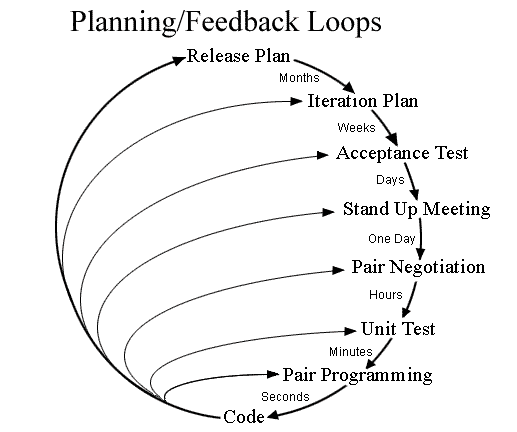
\includegraphics[width=0.6\textwidth]{xp.png}
  \caption{Extreme Programming feedback diagram\cite{xp}}
  \label{fig:xp}
\end{figure}

This methodology proposes a feedback/release cycle as shown in Figure~\ref{fig:xp} and a set of
practices\cite{xp}:

\begin{enumerate}
\item \textit{The planning game}: The scope, priority and date of releases
  should be agreed between business and technical team, adapting them in the
  face of unplanned events. Neither business nor technical parties involved have
  more weight than the other when planning next releases. This is why
  communication is one of the key principles in this methodology. In Alcaudon
  the business team was represented by the advisor, \textit{David Villa Alises},
  and the technical team by the author.
\item Small releases: Every release should be as small as possible providing the
  maximum business value. Alcaudon is released continuously, meaning that it has
  adopted Continuous Deployment\cite{cd} techniques. Every commit pushed to the
  master branch, Travis CI (footnote) launches a continuous delivery pipeline
  that runs tests, builds and publishes an usable version of Alcaudon as docker
  containers and a snapshot version of the libraries to Maven central. This
  practice allows Alcaudon's process to bring value as soon as possible.
  Moreover, it reduces risks, thus contributing to build a more efficient and
  robust system.
\item \textit{Metaphor}: A common language between different participants in the
  project should be use. This makes communication easier and therefore
  misunderstandings are reduced.
\item Simple design: As defined by\cite{xp}, a simple design follows these rules:
  \begin{enumerate}
  \item All tests pass.
  \item There is no duplicated logic.
  \item States every intention important to the programmers.
  \item Has the fewest possible classes, methods and functions.
  \end{enumerate}
  Alcaudon follows these principles. Consequently, the risks associated to
  changes are minimized.
\item Testing: In XP there is a strong bias towards writing tests for all the
  created functionalities, both unit and functional tests. This practice creates
  a stronger confidence in programmers when they need to change their code.
  Alcaudon has been tested broadly, using unit, integration and property based
  testing. Having a good testing coverage has helped to keep developing the
  system with confidence in its correctness, since this project can not be
  easily tested manually.
\item Refactoring: Given the previous principle of \textit{simple design},
  continuous design refinement via refactoring is a key concept in XP.
  Refactoring helps to keep control of complexity iterating over software
  design, reducing risks in future changes. During the development of this
  project, there have been some refactors that improved the design of certain
  modules. Following this principle has been crucial to improve the system's
  architecture.
\item Pair programming: In this methodology there is a preference towards programming
  in pairs. Different points of view can improve the final design and spot
  possible failures that otherwise would have taken longer to detect. This
  principle does not apply to Alcaudon since it is an individual project.
\item Continuous Integration: Code should be integrated and tested every few
  hours. This practice helps to avoid working too long in a big feature, making
  it harder to integrate later. Again, XP is favoring risk reduction with this
  set of practices. As described before, Alcaudon uses Travis CI as continuous
  integration server, for every commit to master the project is built and
  tested.
\item On-site customer: XP accentuates the importance of communications. A
  domain expert, i.e. an user, should be available to answer questions about the
  business and set small scale priorities. Having this person accessible, saves
  time when developers are not familiar with some details about the domain, therefore
  reducing risks.
\item Coding standards: Every project should have coding standards so the
  differences in style among the code written by the team are minimized. An
  example could be a code linter, so if there is a deviation in the defined
  style the programmer will be warned. There are more sophisticated tools to
  define standards, such as code quality measurements tools. These metrics can
  be added in the continuous integration pipeline. if the added code does not
  comply with them, the build is marked as failed. This project uses a code
  linter and advanced compiler warnings (such as unused code, deprecated APIs,
  etc), therefore the coding style is uniform.
\end{enumerate}

\subsection{eXtreme Programming applied to this project}

This section describes the different releases done during the development of
Alcaudon. As it has been stated before, Continuous Deployment has been
implemented, so there has been a production ready release after every code
change. For simplicity this section will describe release cycles with blocks of
features.

\subsubsection{Release 1: State of the art analysis}
\begin{itemize}
\item \textit{Agreed goal}: Distributed data processing systems State of the art analysis.
  \item \textit{Deliverable}: Document describing existing solutions in the
    distributed data processing space as well as recent developments from
    different related conferences such as, VLDB, SIGMOD and OSDI.
\end{itemize}

\subsubsection{Release 2: Technology selection}
\begin{itemize}
\item \textit{Agreed goal}: Given the findings from the previous release,
  investigate suitable technologies to implement a distributed data processing
  system.
\item \textit{Deliverable}: After some investigation and tests two languages
  were chosen, Erlang and Scala. Both implement the actor model. Erlang has been
  proven to be production ready, but according to TIOBE\cite{tiobe} its usage is
  not ample. On the other hand, Scala seems to be quite popular among the data
  processing community. After some discussion with business stakeholders, Scala
  was chosen due to its inter-operability with Java and notoriety among
  developers.
\end{itemize}

\subsubsection{Release 3: Computation, timer, source and sink API definitions}
\begin{itemize}
\item \textit{Agreed goal}: Define the public interface that customers will use
  to implement their computations and timers as well as sources and sinks.
\item \textit{Deliverable}: During this release cycle, communication between the
  different participants in the project was quite productive. A first proposal
  was sent to the domain expert, the advisor in this project. This first version
  did not take into account certain details that were key to the project. Given
  the early feedback, it was possible to react quickly and present a new
  computation API that contained less details about the implementation,
  providing a better abstraction.
\end{itemize}

\subsubsection{Release 4: Dataflow builder development}
\begin{itemize}
\item \textit{Agreed goal}: Develop a first dataflow builder version where the
  user can define a dataflow topology.
\item \textit{Deliverable}: During this release an usable dataflow builder was
  delivered. Alcaudon users were able to build their own computation topologies.
  This allowed to start testing how usable the interface was and with the given
  feedback improve the initial designs.
\end{itemize}

\subsubsection{Release 5: First computation execution engine version development}
\begin{itemize}
\item \textit{Agreed goal}: Implement the first version for the computation
  execution engine.
\item \textit{Deliverable}: Since Dataflow builder was developed during the previous
  release, the next natural step was to implement the computation executor.
  During this release a simplified engine version was released, making possible
  to test simple computations.
\end{itemize}

\subsubsection{Release 6: Computation execution guarantees development}
\begin{itemize}
\item \textit{Agreed goal}: Implement means to provide fault-tolerant computation executions.
\item \textit{Deliverable}: One of the Alcaudon goals is to be fault-tolerant.
  The outcome of this release cycle was fully tested computation engine that
  complies with the fault-tolerant agreed requirements.
\end{itemize}

\subsubsection{Release 7: Timer execution engine development}
\begin{itemize}
\item \textit{Agreed goal}: Implement fixed and watermark based timers.
\item \textit{Deliverable}: Alcaudon works with unbounded data-sets, hence a way
  to emit partial results should be provided. In this release, fixed timers and watermark
  timers were released. Watermarks were developed using CRDT's.
\end{itemize}

\subsubsection{Release 8: Generic serialization library development}
\begin{itemize}
\item \textit{Agreed goal}: Develop generic serialization library for Algebraic
  Data Types.
\item \textit{Deliverable}: Data travels around Alcaudon as an array of bytes.
  There are many serialization formats to transform high level entities to
  binary data. However, for simplicity, a generic serialization library has been
  developed. This library is able to, given an Algebraic Data Type, create a
  serializer/de-serializer using scala implicit induction during compile time.
\end{itemize}

\subsubsection{Release 9: Stream entity implementation}
\begin{itemize}
\item \textit{Agreed goal}: Implement a Stream representation so data can be
  published and consumed from it. Published data should be durable.
\item \textit{Deliverable}: Since computations subscribe to streams, in this release a
  durable stream representation was implemented. This allows consumers and publishers to
  consume and publish stream records. During this release, given the changes
  that appeared during the design of the stream entity, some refactors in the
  computation execution engine were done.
\end{itemize}

\subsubsection{Release 10: Library manager implementation}
\begin{itemize}
\item \textit{Agreed goal}: Implement a subsystem that enables dynamic load of
  arbitrary user code into remote Alcaudon workers.
\item \textit{Deliverable}: A module to load arbitrary user code was developed.
  It is backed by a cloud object storage\footnote{https://aws.amazon.com/s3/},
  and allows dynamic load of user code.
\end{itemize}

\subsubsection{Release 11: Distributed architecture design}
\begin{itemize}
\item \textit{Agreed goal}: Design a resilient distributed architecture that
  allows remote work distribution for the system.
\item \textit{Deliverable}: During this release some requirement changes were brought
  by the business side due to a bug in the stream implementation. Given the urgency
  of those changes, just a partial design was done.
\end{itemize}

\subsubsection{Release 12: Distributed architecture implementation}
\begin{itemize}
\item \textit{Agreed goal}: Finish the first design for the distributed
  architecture and implement a prototype.
\item \textit{Deliverable}: In this release, a first version for the distributed
  architecture was developed. The idea was to keep developing during the next
  release cycles.
\end{itemize}

\subsubsection{Release 13: Implement job scheduling policy}
\begin{itemize}
\item \textit{Agreed goal}: Implement computation scheduling to distribute the
  dataflow topology in the most optimal possible configuration.
\item \textit{Deliverable}: Due to the time constraints, during this release it
  was decided to use available tools to solve the flexible job-shop scheduling
  problem. In this case, a set of optimization tools provided by Google was
  used.
\end{itemize}

\subsubsection{Release 14: Implement tools that allow monitoring the system}
\begin{itemize}
\item \textit{Agreed goal}: Implement tools or adopt external tools that allow
  observing the behavior of the system.
\item \textit{Deliverable}: After some investigation it was agreed to used both
  an external system to facilitate observability, Prometheus, and implement some
  tools to track how the system is performing.
\end{itemize}

\subsubsection{Release 15: implement some sources and sinks}
\begin{itemize}
\item \textit{Agreed goal}: Provide some default implementations of sources and
  sinks, such as TCP sockets or Twitter streaming api.
\item \textit{Deliverable}: During this release the agreed goals were implemented. Given
  that the system needed some improvements, this latest release was used also to refactor
  some modules of the system to give them more reliability.
\end{itemize}

\section{Development technologies}

There are many technologies available to develop information systems. Different
paradigms, different environments, etc. For Alcaudon, working with the JVM
was the perfect match. It is one of the most advanced language virtual
machines in the market, with outstanding implementations such as
OpenJDK\footnote{http://openjdk.java.net/} or
Zing\footnote{https://www.azul.com/products/zing/virtual-machine/}. The
available ecosystem of tools and libraries covers many domains. There are
multiple implementations for the state of the art data structures used in this
project, such as cuckoo filters\cite{cuckoo}. Another reason to choose the JVM
was the inter-operability between different languages such as Scala and Java.
Scala has been chosen as the principal programming language.
It is an hybrid language that allows programmers to use functional and object
oriented programming paradigms. The compelling aspect of this design is that it
allows the combination of the best of both worlds. It provides tools to work
with functional constructs such as monadic composition or use more object
oriented tools such as traits.

In the database space, \textit{Cassandra} has been chosen as the principal data store due
to it is designed with high availability and scalability in mind. This choice
provide good grounds to guarantee data durability within the system. For storing
time series data, \textit{Prometheus} has been chosen due to its high scalability and
performance querying historic data.

Another tool used in the development Alcaudon has been \textit{TravisCI}, a
cloud continuous integration service. Using a service that is fully integrated
with git facilitated the set-up of the CD pipeline easier.

\section{Tools}

In this section the tools used to develop Alcuadon will be presented. 

\subsection{Hardware}

The only physical hardware used to develop this project has been a laptop. For
deploying the system, Amazon Web Services has been used. All the incurring costs
for testing have been assumed by the author of this project.

\begin{itemize}
  \item Dell XPS 13 with Intel\textregistered Core\texttrademark i5 2.5GHz
    processor 8GB RAM DDR3 and 128GB SSD hard drive.
  \item Amazon Web Services provided servers with different specifications.
\end{itemize}

\subsection{Software}

\begin{itemize}
  \item Operating Systems
    \begin{itemize}
        \item Debian 8 Jessie\footnote{https://www.debian.org/index.es.html}.
          Operating system used to develop the system and the documentation.
        \item CoreOS\footnote{https://www.coreos.com/}. Minimal linux operating
          system that supports container systems out of the box. Used to deploy
          Alcaudon.
    \end{itemize}

  \item Languages
    \begin{itemize}
      \item Scala\footnote{https://www.scala-lang.org/}. Hybrid Functional and
        Object Oriented programming language used to develop the system.
      \item \LaTeX{}\footnote{https://www.latex-project.org/}. Language used to
        write this document.
    \end{itemize}

  \item Frameworks, libraries and databases
    \begin{itemize}
      \item Akka\footnote{https://akka.io}. Toolkit to develop actor based
        systems. Most of the system relies on the actor model. The following
        extensions have been used:
        \begin{itemize}
        \item akka-cluster
        \item akka-persistence
        \item akka-distributed-data
        \end{itemize}
      \item Shapeless\footnote{https://github.com/milessabin/shapeless}. Generic
        programming for Scala used to develop generic serializers.
      \item Apache Cassandra\footnote{http://cassandra.apache.org/}. Open source
        database aimed for scalability.
      \item Scala Graph\footnote{http://www.scala-graph.org/}. Graph data
        structure implementation for Scala.
      \item
        CuckooFilter4j\footnote{https://github.com/MGunlogson/CuckooFilter4J}.
        High performance Java implementation of a Cuckoo filter.
      \item ScalaCheck\footnote{https://www.scalacheck.org/}. Property based
        testing library for Scala.
      \item ScalaTest\footnote{http://www.scalatest.org/}. Testing framework for
        Scala.
      \item Kryo\footnote{https://github.com/EsotericSoftware/kryo}. Fast efficient serialization
        framework for the JVM.
      \item Prometheus\footnote{https://github.com/EsotericSoftware/kryo}. Open
        source time series database used for monitoring.
      \item Google Optimization
        Tools\footnote{https://github.com/google/or-tools}. Google Optimization
        Tools (OR-Tools) is a fast and portable software suite for solving
        combinatorial optimization problems. Used for job scheduling.
    \end{itemize}

  \item Tools
    \begin{itemize}
      \item sbt\footnote{http://www.scala-sbt.org/}. Build tool for Scala.
      \item Emacs \footnote{https://atom.io/}. Text editor used to program the system.
      \item Git\footnote{https://git-scm.com/}. Distributed version control system.
      \item TravisCI\footnote{https://www.travis-ci.org/}. Cloud continuous integration service.
      \item Docker\footnote{https://www.docker.com/}. Linux container runtime.
      \item Grafana\footnote{https://grafana.com/}. Open platform for analytics and monitoring.
    \end{itemize}

\end{itemize}

\chapter{Architecture}
\label{chapter:architecture}

Alcaudon's architecture will be described in this chapter following a top-down
approach. Firstly, a general description of the different components of the system
will be explained. Finally, each of the components will be described more thoroughly.

\section{General description}

Alcaudon's platform is composed by 3 main units.

\begin{itemize}
\item \textbf{Alcaudon library}: This is the main interface between users
  and the system. In order to use Alcaudon it is necessary to have access to a
  cluster with a coordinator and computing nodes. This interface is provided as
  a library containing the tools to build dataflows, the interfaces to implement
  user defined stream computations and the tools to connect with a particular
  cluster. Since the computations are potentially infinite, the operations
  performed against the cluster are asynchronous, returning an id associated
  with the created operation.
\item \textbf{Coordinator node}: This is the main component of the system. It
  coordinates the life cycle of the different components of the cluster such as
  the computing nodes. It is also responsible of performing the scheduling of
  the user defined dataflows given the resources provided by the computing
  nodes. Finally, it is the interface between the cluster and the users, where
  they deploy their dataflow topologies.

\item \textbf{Computing nodes}: These nodes are in charge of executing the
  actual computations provided by Alcaudon's users. These nodes take care of
  storing intermediate results published to streams. They register dynamically
  to the cluster contacting the coordinator node. A deployment can be composed
  from one computing node up to thousands, as needed. Each of these nodes
  provides certain resources to the system, known as \textit{computation slots}.
  The number of slots is configurable, but they correlate with the number of
  available CPU's in the underlying hardware.
\end{itemize}

A high level overview of the system can be seen in
figure~\ref{fig:architecture}. The majority of the parts of the system have been
modeled as Actors. As it was stated previously it is a very good fit for this
kind of applications. Where possible, object oriented design patterns\cite{gof}
such as \textbf{builder} or \textbf{factory} have been used. However, functional
programming constructs such as monads\cite{monads}, type
classes\cite{typeclasses} or Algebraic Data Types have been used more widely.

Once the different parts of the system have been presented, they will be
inspected in detail.

\begin{figure}
  \centering
  
\includegraphics[width=1\textwidth]{architecture.pdf}
  \caption{Alcaudon architecture schema}
  \label{fig:architecture}
\end{figure}

\section{Alcaudon library}

In the first place, the user facing interface will be presented in detail. In order
to create a streaming data processing pipeline, or dataflow topology as it has
been defined during all this document, users should provide their business
logic. To achieve this goal, Alcaudon provides certain interfaces so users
just need to care about their code. These interfaces are available as a library
that can be found at at Sonatype OSSRH \footnote{http://central.sonatype.org/pages/ossrh-guide.html}.

\begin{figure}
  \centering
  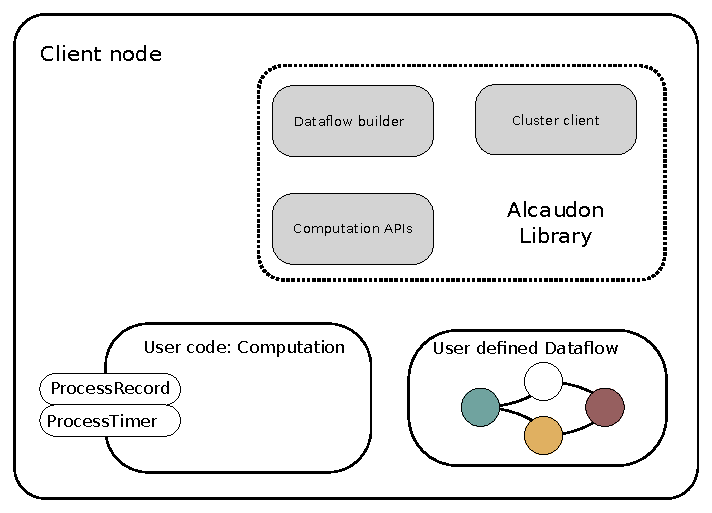
\includegraphics[width=0.6\textwidth]{client.pdf}
  \caption{Alcaudon library}
  \label{fig:library}
\end{figure}

This library is composed of three modules as it is shown in figure~\ref{fig:library}:

\begin{itemize}
\item Computation API's: Interface that users should implement in order to
  create computations.
\item Dataflow builder: This component is used to build dataflow topologies and
  later on submit the to the cluster coordinator.
\item Cluster client: Communication layer between clients and Alcaudon clusters.
  It handles all the operations needed to submit custom code to the cluster as well
  as the stream processing pipeline definition.
\end{itemize}

\subsection{Computation API's}

\begin{figure}[!h]
  \begin{center}
  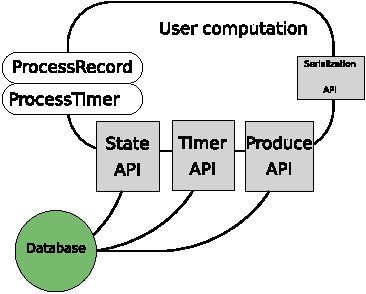
\includegraphics[width=0.5\textwidth]{libraryApi.pdf}
  \caption{Alcaudon computation API's}
  \label{fig:apis}
  \end{center}
\end{figure}

As explained before, in order to create custom computations to process unbounded
data-sets in Alcaudon, it is necessary to implement an interface. The interface
is listed in~\ref{code:computation}. This interface gives access to the
abstractions provided by the system as represented in figure~\ref{fig:apis}. As
it can be observed, there are two methods to be implemented;
\lstinline[columns=fixed]{def processRecord(record: Record): Unit} and \lstinline[columns=fixed]{def processTimer(timer: Timer): Unit}.

\begin{lstlisting}[language=scala, frame=trBL, label=code:computation, float=ht, caption = {Computation API's}]
trait Computation
    extends ProduceAPI
    with TimerAPI
    with StateAPI
    with SerializationAPI
    with RuntimeContext {
  ...
  def processRecord(record: Record): Unit
  def processTimer(timer: Timer): Unit
  ...
}
\end{lstlisting}

\begin{lstlisting}[language=scala, frame=trBL, label=code:computationExample, float=ht, caption = {Computation example}]
class Windower extends Computation {
  // Counts the number of records per key
  def processRecord(record: Record): Unit = {
    val bucketCount: Int = deserialize(get(record.key))
    set(record.key, serialize(bucketCount + 1))
    setTimer(FixedRecurrentTimer(record.key, 5.minutes))
  }

  // Timers are triggered and produce records with the count of keys.
  def processTimer(timer: Timer): Unit = {
    val bucketCount: Int = deserialize(get(timer.tag))
    produceRecord("windowsCount", RawRecord(get(timer.tag), timer.timestamp))
  }
}
\end{lstlisting}

These methods represent the main entry point into user code, hooked in reaction to
record receipt and timers expiration. These constitute the application logic.
Within the execution of these methods, Alcaudon provides different functions to
work with persistent state, publish new records to streams, set timers or
serialize arbitrary data types. In Alcaudon, each computation can subscribe to
multiple sources represented as streams. Data travels in its simplest form,
as an array of bytes. One specific example can be found in listing~\ref{code:computationExample}.

\begin{figure}
  \begin{center}
    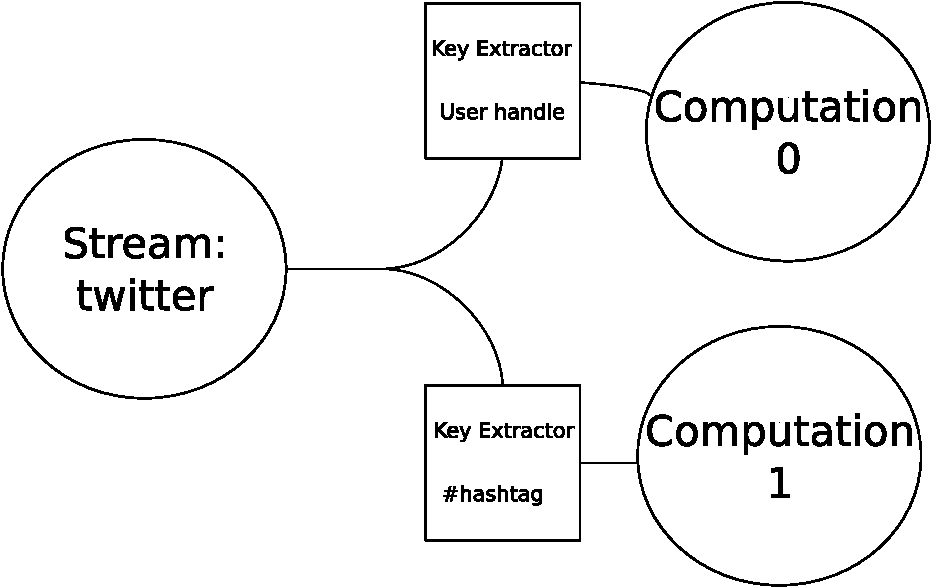
\includegraphics[width=0.5\textwidth]{keypartitioning.pdf}
    \caption{Alcaudon record key assignment}
    \label{fig:keypartitioning}
  \end{center}
\end{figure}

However, for each stream subscription users should provide a key extraction
function, this process shown in figure~\ref{fig:keypartitioning}. Having a key
per record allows the implementation of parallelization strategies such as key
partitioning. Therefore, every record emitted by one of the subscribed sources,
an instance of the class \lstinline[columns=fixed]{Record} listed
in~\ref{code:records}, will be injected with the call to
\lstinline[columns=fixed]{processRecord}.

\begin{lstlisting}[language=scala, frame=trBL, label=code:records, float=ht, caption = {Record classes}]
case class RawRecord(value: Array[Byte], timestamp: Long) {
  val id = UUID.randomUUID().toString
}
case class Record(key: String, rawRecord: RawRecord) {
  val value = rawRecord.value
  val timestamp = rawRecord.timestamp
  val id = UUID.randomUUID().toString
}
\end{lstlisting}

Timers are the other possible trigger for user defined code execution. In
Alcaudon there are three types of timers:

\begin{itemize}
\item \textit{Fixed timers}: This kind of timers are triggered once at a
  specific wall time.
\item \textit{Recurrent fixed timers}: This timer resembles the previous timers
  with the exception that it is executed recurrently. I.E., every five minutes.
\item \textit{Watermark timers}: This timer tries to estimate the point where all
  the events up to certain window have been consumed by the system and execute
  then. The mechanism and algorithm used to implement them will be explained
  later.
\end{itemize}

When a timer is executed it has as a parameter an instance of the class Timer
listed in ~\ref{code:timers}. These constructs are key to the domain of unbounded
data-sets due to their very nature. A mean to emit partial results is needed, so
this is the mechanism provided by Alcaudon to emit results.

\begin{lstlisting}[language=scala, frame=trBL, label=code:timers, float=ht, caption = {Timer class}]
  case class Timer(tag: String, timestamp: Long)
\end{lstlisting}

\subsection{Dataflow builder}

Once the computations are implemented, users need a way to build the dataflow topologies.
To achieve this goal, the system provides a dataflow builder. Using this instrument,
users are able to define dependencies among the computations in the system.
These main entities that can be used in Alcaudon are:

\begin{itemize}
  \item \textit{Sources}: Sources bring external data into the system. Some
    examples could be a TCP/IP socket, Twitter streaming API, Apache Kafka,
    Zeromq, etc.
  \item \textit{Computations}: Computations are user defined business logic.
  \item \textit{Streams}: Streams represent the delivery instrument between
    different computations in Alcaudon. Computations subscribe to one or more
    streams and publish to zero or more streams. Alcaudon guarantees the
    delivery of records along these streams.
  \item \textit{Sinks}: Sinks are a special kind of streams, providing a way to
    publish data to external systems such as http endpoints or databases. They
    are useful to project final results.
\end{itemize}

Alcaudon dataflow builder is defined in listing~\ref{code:builder}. Dependencies
are checked, thus if one computation depends or publishes into an unknown stream,
the dataflow definition will be considered invalid. Internally, defined
dataflows are represented as a \acf{DAG}~\ref{fig:dataflowbuilder}. In this graph, vertices
represent computations and streams while edges represent the dependencies
between them or how data flow along the system. Considering that the execution
of the dataflow is performed remotely and computations are arbitrary user code,
computations are represented as their fully qualified name inside the \acs{JVM}
classpath. Using this fully qualified name in combination with dynamic class
loaders, it is possible to load code dynamically. In conclusion, with this builder
it is possible to create declarative representations of Alcaudon data pipelines.
This representation abstracts away all the details about in which compute nodes
code will run or how parallelism will be implemented. This approach is quite
similar to how Free Monad\cite{freemonad}, SQL or Prolog works.

\begin{lstlisting}[language=scala, frame=trBL, label=code:builder, float=ht, caption = {Alcaudon's DataflowBuilder}]
DataflowBuilder(dataflowName: String)
  .withSource(sourceName: String, sourceDescription: SourceDescription)
  .withComputation(computationName: String,
    computation: Computation,
    outputStreams: Set[StreamID],
    AlcaudonInputStream(StreamID)(keyExtractor: Array[Byte] => String)*
  .withSink(sinkName: String, sinkDescription: SinkDescription)
  .build()
\end{lstlisting}

\subsection{Cluster client}

\begin{figure}
  \centering
  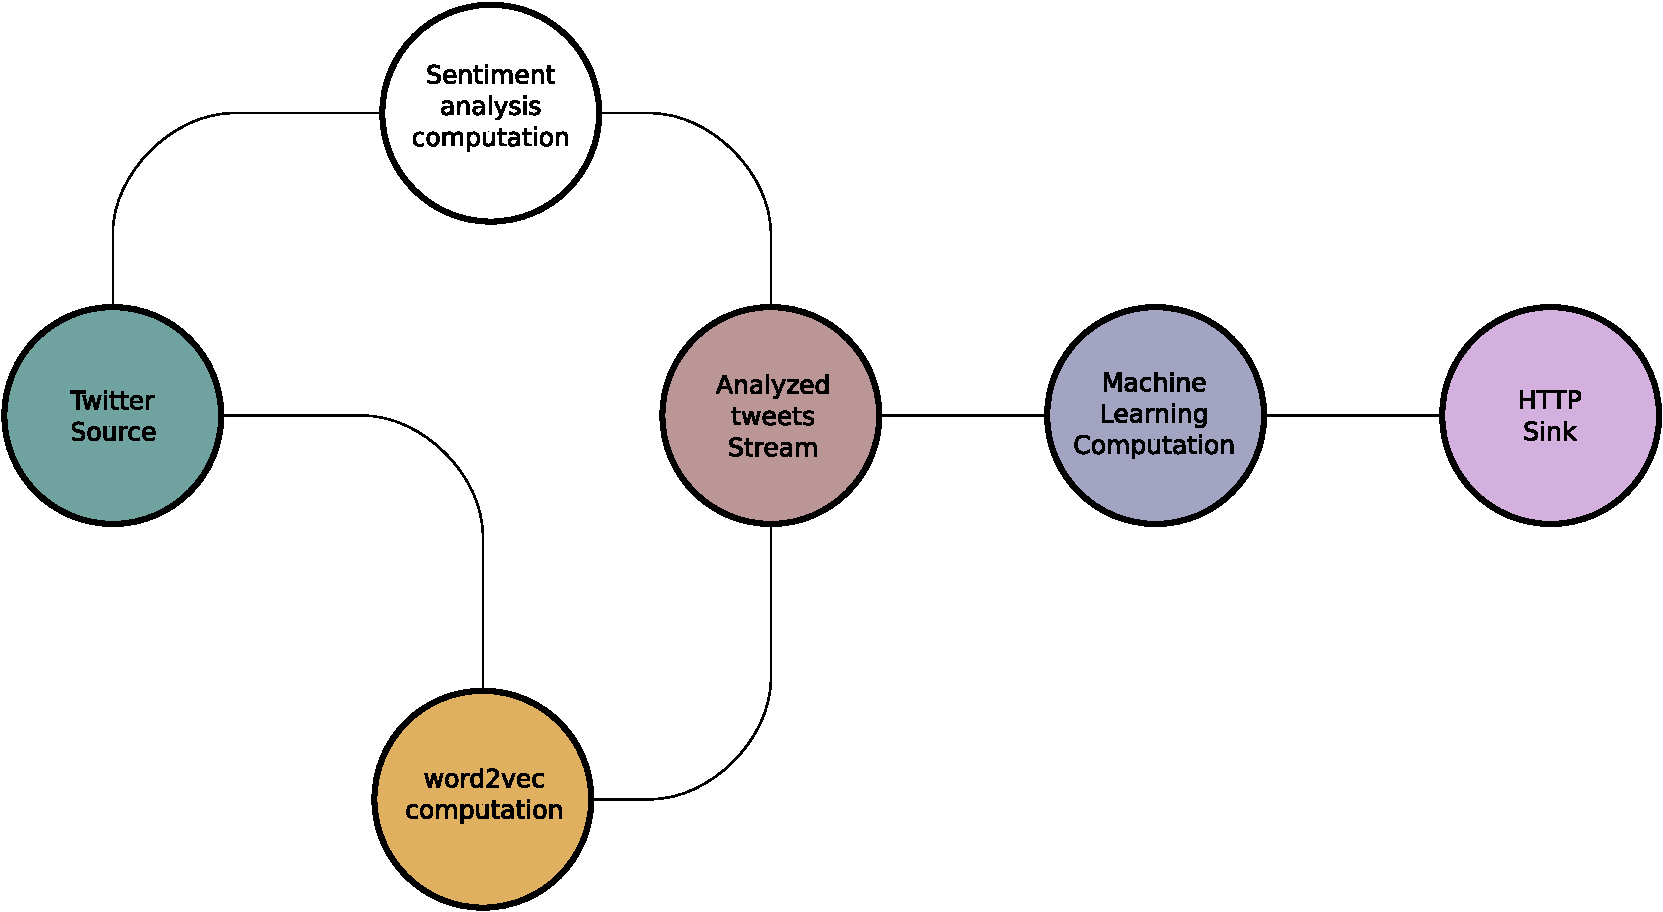
\includegraphics[width=0.8\textwidth]{dataflowbuilder.pdf}
  \caption{Dataflow \acs{DAG} example}
  \label{fig:dataflowbuilder}
\end{figure}

Once the computations and topology have been defined, some machinery is required
in order to execute them in an Alcaudon cluster
(figure~\ref{fig:dataflowbuilder}). In Alcaudon library there are the tools
needed to connect to an existing cluster and perform certain operations. The
available operations are listed in table~\ref{tab:operations}. Creating a
dataflow pipeline is an asynchronous operation, returning a DataflowPipeline
\acf{UUID} that identifies the created pipeline. With this \acs{UUID} it is
possible to perform some operations over the pipeline.

\begin{table}[hp]
\centering
\begin{tabular}{|l|l|l|}
\hline
\textbf{Action} & \textbf{Parameters} & \textbf{Returned info} \\ \hline
\begin{tabular}[c]{@{}l@{}}Send Dataflow topology\end{tabular}  & DataflowGraph and \acs{jar}s & DataflowPipeline UUID \\ \hline
\begin{tabular}[c]{@{}l@{}}Get DataflowJob execution info\end{tabular} & DataflowPipeline UUID & DatflowPipelineStatus \\ \hline
\begin{tabular}[c]{@{}l@{}}Stop DataflowJob execution\end{tabular} & DataflowPipeline UUID & DatflowPipelineStatus \\ \hline
\end{tabular}
\caption{Available cluster management operations}
\label{tab:operations}
\end{table}

In order to understand better how Alacaudon dataflow pipeline creation works, it
will be explained more thoroughly. This operation is divided into two phases,
first user code libraries are uploaded. Once the libraries are uploaded the
actual dataflow pipeline is created. Uploading user libraries is needed so
computing nodes can have access to user business logic. The number of computing nodes that
can access concurrently to these user libraries depends on the deployment,
reaching up to thousands in some cases. To avoid any scaling problems, libraries
are stored into an object storage service. In this case, they are stored in
Amazon S3\footnote{https://aws.amazon.com/s3/}. These services usually provide a
way to avoid the need to first upload the data to a backend server in order to
get access to credentials to later on upload data to an object storage services.
This is achieved using pre-signed URL's, based on a temporary token generated
using service credentials and a timestamp. In Alcaudon, cluster clients
request the creation of a dataflow pipeline. As a response, a pre-signed URL
alongside an UUID that identifies the operation is returned by the cluster
coordinator. Once cluster clients have the URL, they can use it to upload user
code directly to the object storage service. With the user code uploaded, the
next step is to create the actual Dataflow pipeline. Given the returned UUID a
request is done to cluster coordinator in order to finish the dataflow pipeline
creation. The communication is performed using akka remote that allows
communications with remote actor systems.The whole process is represented as a
sequence diagram in figure~\ref{fig:pipelinecreation}. This process is performed
transparently by the library from users perspective.

\begin{figure}[!h]
  \centering
  \scalebox{0.6}{
    \input{figures/dataflowcreation.latex}
  }
\caption{Sequence diagram for Dataflow pipeline creation}
\label{fig:pipelinecreation}
\end{figure}

\subsection{Serialization API}

Programmers are used to work with high level abstractions in order to model the
domain they are working on. As it has been described previously, records in
Alcaudon are a tuple of a key and an array of bytes. Given this fact, a way to
work with high level entities is needed. There are many options to serialize and
deserialize data available, such as JSON, Protocol Buffers, etc. Alcaudon users
are free to use the serialization format they prefer. However, to ease working
with the platform, a generic serialization library typeclass is provided. This
library is capable of, given an \acs{ADT} generate automatically serializers and
deserializers during compile time. This is possible thanks to an advanced Scala
feature, implicits resolution, and one library for generic programming,
Shapeless. \acs{ADT}s are a functional programming concept that allow data
representation in terms of \textit{products} and \textit{sums} of types. A
\textit{product} is a combination of different types $(A \& B)$. On the other
hand a \textit{sum} is an alternation of different types $(A | B)$. In Scala,
\acs{ADT} are expressed as case classes and traits as shown in
listing~\ref{code:adt}.

\begin{lstlisting}[language=scala, frame=trBL, label=code:adt, float=ht, caption = {\acs{ADT} example}]
  sealed trait Message // Message = (Tweet | Account)
  case class Tweet(user: String, id: Int, timestamp: Long) extend Message // Tweet = (String & Int & Long)
  case class Account(name: String, age: Int) extend Message // Account = (String & Int)
\end{lstlisting}

Taking this into account, case classes could be represented as lists of types,
in \lstinline[columns=fixed]{Tweet} example it can be summarized as a list of
three types, \lstinline[columns=fixed]{String & Int & Long}. Shapeless allows
to represent case classes as a \acf{HList} of types working with them
as they are regular types. Once it is possible to encode \acs{ADT}s as
\acs{HList} of types a tool to convert that generic representation into
a serializer is needed. To achieve this goal, Scala implicit type system is the
answer. Scala implicits are a way to provide certain parameters marked as
implicits to functions without the need to pass them explicitly. Scala compiler has
a set of strict rules\footnote{http://docs.scala-lang.org/tutorials/FAQ/finding-implicits.html}
to look for implicit parameters. The interesting part comes when functions with implicit
parameters use parametric polymorphism, such as Alcaudon's serialization typeclass
listed in~\ref{code:typeclass}.
\begin{lstlisting}[language=scala, frame=trBL, label=code:typeclass, float=ht, caption = {Serializer-Deserializer typeclass}]
trait TypeInfo[T] {
  def serialize(obj: T)(implicit output: DataOutput): DataOutput
  def deserialize(t: DataInput): T
}
\end{lstlisting}

It is possible to write an implicit rule that creates a
\lstinline[columns=fixed]{TypeInfo} for \lstinline[columns=fixed]{(A, B)} given
\lstinline[columns=fixed]{TypeInfo} for \lstinline[columns=fixed]{A} and
\lstinline[columns=fixed]{B}. This feature is provided by Scala implicit
resolution mechanism that works as an inductive solver. Therefore, if
\lstinline[columns=fixed]{TypeInfo} instances for every basic data type are
implemented it is possible to write rules for \acs{HList} of
\textit{products}. As a result, Scala compiler will be able to inductively
generate \lstinline[columns=fixed]{TypeInfo} instances for any \acs{ADT}
during compile time.

\begin{lstlisting}[language=scala, frame=trBL, label=code:generation1, float=ht, caption = {Serializer-Deserializer typeclass using parametric polymorphism}]
  implicit def genericObjectEncoder[A, H <: HList, O <: HList](
      implicit generic: LabelledGeneric.Aux[A, H],
      repFormat: Lazy[TypeInfo[H]],
      keys: Keys.Aux[H, O]
  ): TypeInfo[A] =
    new TypeInfo[A] {
      def serialize(v: A)(implicit output: DataOutput) = {
        repFormat.value.serialize(generic.to(v))
      }

      def deserialize(input: DataInput) = {
        generic.from(repFormat.value.deserialize(input))
      }
    }
\end{lstlisting}

Details about how rules for generic types and \acs{HList} are implemented can be
found in listings ~\ref{code:generation1} and ~\ref{code:generation}. For
objects of type T, Shapeless is used in order to obtain its encoding as an
\acs{HList}; this is done in \lstinline[columns=fixed]{genericObjectEncoder}.
With this encoding, it is possible to call the serializer for \acs{HList}s in
implicit method \lstinline[columns=fixed]{hListFormat}. In this method, using
recursive induction, a type class for each type is searched and combined, thus
creating a serializer for the \acs{HList} then for the type T.

\begin{lstlisting}[language=scala, frame=trBL, label=code:generation, float=ht, caption = {Serializer-Deserializer typeclass for \acs{HList}}]
  implicit def hListFormat[Key <: Symbol, Value, Remaining <: HList](
      implicit key: Witness.Aux[Key],
      lazyTih: Lazy[TypeInfo[Value]],
      lazyTit: Lazy[TypeInfo[Remaining]]
  ): TypeInfo[FieldType[Key, Value] :: Remaining] =
    new TypeInfo[FieldType[Key, Value] :: Remaining] {
      ...
      def serialize(hlist: FieldType[Key, Value] :: Remaining)(
          implicit output: DataOutput) = {
        val headOutput = tih.serialize(hlist.head)
        tit.serialize(hlist.tail)(headOutput)
      }

      def deserialize(input: DataInput) = {
        val head = tih.deserialize(input)
        val tail = tit.deserialize(input)
        field[Key](head) :: tail
      }
    }
\end{lstlisting}

As an interesting note, this part of the system has been tested using property
based testing\cite{quickcheck}. Using this kind of testing helped to spot
otherwise difficult bugs to detect.

\section{Computation node}

\begin{figure}[!h]
  \centering
  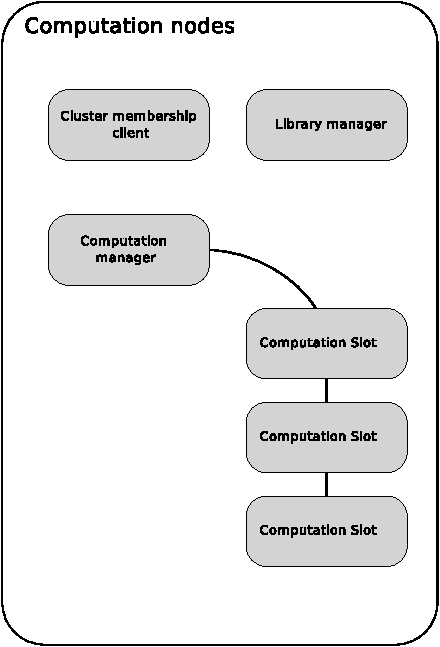
\includegraphics[width=0.5\textwidth]{computationnode.pdf}
  \caption{Computation node modules}
  \label{fig:computationnode}
\end{figure}

Once Alcaudon library has been described, computation node architecture design
will be presented. This component is in charge of executing the actual
computations. A high level overview of this component can be found in
figure~\ref{fig:computationnode}. It is composed of four modules:
\begin{itemize}
\item \textit{Cluster membership client}: This module is in charge of handling
  the communications with the cluster coordinator. It announces the availability
  of a new computing node once it is up and ready to receive work. It announces
  the intention to leave the cluster so it is possible to re-schedule work into
  other computing nodes gracefully. Another responsibility of this module is to
  send heartbeats to the cluster coordinator in order to assure that the node is
  healthy.
\item \textit{Library manager}: Library manager handles the download of user
  defined code as well as loading it into the process classpath dynamically.
  It downloads the contents from the object storage into disk, so content is
  just downloaded once per computing node. Once the \acs{jar}'s are downloaded,
  they are loaded into a controlled user \acs{JVM} classpath. This avoids
  classpath collisions, i.e. different computations use a library but with
  different versions. This process is described as a sequence diagram in
  figure~\ref{fig:librarymanagement}.
\item \textit{Computation manager}: Computation manager is responsible for
  deploying computations and streams into the computing node. A computing node
  has a limited amount of resources, and in Alcaudon they are represented as
  \textit{computation slots}. \textit{Computation slots}
  define how many computations can run in parallel. Usually, the number of
  available slots is correlated with underlying physical hardware in which the
  computing node is running. This value is configurable, thus Alcaudon does not
  impose any limits in the number of \textit{computation slots}. However, it
  is recommended to use values near the number of available CPU's. During
  the membership phase, coordinator node is informed about the number
  of usable slots. This information is used during scheduling. When a new
  job is scheduled to be run in a certain node, the computation manager
  is the point of communication between the coordinator and the node.
  It deploys the scheduled streams and computations and supervises them,
  using actor supervision.
\end{itemize}

\begin{figure}[!h]
  \centering
  \scalebox{0.45}{
    \input{figures/librarymanagement.latex}
  }
  \caption{Alcaudon computing node LibraryManager}
  \label{fig:librarymanagement}
\end{figure}

Once a high level overview of this sub-system has been done, a more
comprehensive description of the modules will be undertaken.

\subsection{Cluster membership}

Computing nodes need a procedure to join existing Alcaudon's clusters
dynamically. This feature allows scaling up when more computing resources are
needed and down-scaling when there are over capacity. Cluster membership is a
wide topic and it has many corner cases. Alcaudon uses akka to leverage all the
complexities of managing cluster membership. It provides a failure detector,
where nodes belonging to the cluster monitor each other sending heartbeats in
order to detect unreachable nodes. Heartbeat arrival time is interpreted by an
implementation of The Phi Accrual Failure Detector\cite{phifailure}.

\begin{figure}[!h]
\begin{center}
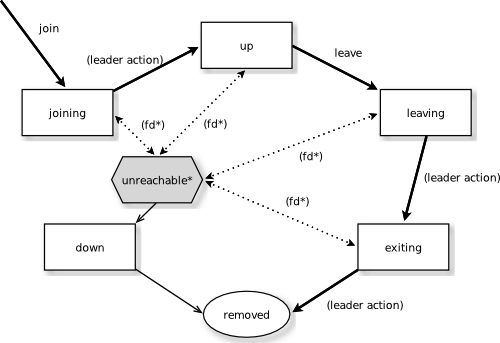
\includegraphics[width=0.7\textwidth]{membershipcluster.png}
\caption{Cluster membership states}
\label{fig:statescluster}
\end{center}
\end{figure}

In figure~\ref{fig:statescluster} the different states in which a cluster node
can be are illustrated. Alcaudon uses this mechanism in order to register new
nodes into the cluster using seed nodes. After joining the cluster, computation
nodes send a message to cluster coordinator in order to signal their
availability to receive new computations(\ref{code:noderegistering}).

\begin{lstlisting}[language=scala, frame=trBL, label=code:noderegistering, float=ht, caption = {Compute node registration}]
def register(member: Member): Unit =
    context.actorSelection(RootActorPath(member.address) / "user" / "coordinator") !
      ComputationNodeRegistration(member.id)
\end{lstlisting}

In order to shut-down nodes neatly, a protocol to leave Alcaudon clusters is
needed. This protocol is described in sequence diagram shown in
figure~\ref{fig:stopprotocol}.

\begin{figure}[!h]
  \centering
  \scalebox{0.45}{
    \input{figures/exitnode.latex}
  }
  \caption{Computation node stop protocol}
  \label{fig:stopprotocol}
\end{figure}

\subsection{Computation manager}

As exposed before, computation manager is responsible for deploying and
supervising computations and streams. In order to deploy computations and
streams, the addresses of each of them are needed. To accomplish this
goal, akka location transparency mechanism is used. Akka gives a logical address
to each actor deployed into the system. Having this address allows sending
messages between actors. The translation between the logical address and the
physical address is done transparently by akka. Once this detail is
clarified, deployment process will be described. Cluster Coordinator, as
described in previous subsections, schedules provided dataflow topologies among
the available computing nodes. First, cluster coordinator sends a request to a
computing node asking to deploy certain computations and streams. When the computing
node responds with an acknowledgment, the computation is deployed. The next
step is to start a ComputationExecutor actor for each computation in the request
as well as Stream actors. Once these actors have been started, their logical
addresses are communicated to other members that belong to the same dataflow via
\acs{CRDT}. Using this approach avoiding centralized knowledge for the location
of different computations allows better scalability and resilience. One of the
drawbacks of this approach is an increase in the complexity of ComputationExecutor
actors. Finally, computation manager sends back a message to the coordinator
informing that the deployment has finished. The whole process is represented as
a sequence diagram in figure~\ref{fig:librarymanagement}.

\begin{figure}[!h]
  \centering
  \scalebox{0.45}{
    \input{figures/deployment.latex}
  }
  \caption{Computation deployment sequence diagram}
  \label{fig:deployment}
\end{figure}

\subsection{Computation executor}

When computations are deployed, they are ready to process incoming records from
different sources and streams. One of the goals of the system is to provide
exactly once record processing semantics. In order to implement exactly once
semantics guarantees Alcaudon process records and timers in an idempotent
manner. The algorithm to provide these guarantees can be summarized as follows.

When a new record arrives into a computation the next steps are performed:
\begin{enumerate}
  \item Using duplication detection logic, records are checked to avoid duplicates.
  \item User defined code is run for the received record. This execution can
    result in pending changes to timers, state or downstream productions.
  \item Pending changes are saved into the database.
  \item An acknowledgment is sent back to senders.
  \item Pending new records are sent.
\end{enumerate}

Since storing the result of every new record processing could be costly, the
above operations can be grouped into batches optimizing the process. Records are
sent until the sender gets an acknowledgment, meaning that in reality records
are sent at least once, but the computations are idempotent.

\begin{lstlisting}[language=scala, frame=trBL, label=code:computationState, float=ht, caption = {Alcaudon internal computation state}]
case class ComputationState(kv: Map[String, Array[Byte]],
                              timers: Map[String, Timer],
                              bloomFilter: CuckooFilter[String],
                              var latestWatermark: Long = 0,
                              var processedRecords: Long = 0,
                              var failedExecutions: Long = 0)
\end{lstlisting}

In order to understand better how Alcaudon implements this logic, it will be
explained in depth. Alcaudon uses the actor model widely, computations are not
an exception. One powerful feature provided by Akka is persistent actors. This
extension enables stateful actors to persist their internal state so it can be
recovered in the case of a failure or a cluster migration. Alcaudon uses this
extension alongside with Apache Cassandra\footnote{Apple has a cluster with over
  75000 nodes storing 10 PB of data} as data store. User code can work with
persistent state, create timers or produce records using Alcaudon \acs{API}'s,
that generates state that should be handled by computation actors. Internal
state contains persistent state from the computations executed, timers and
meta-information(~\ref{code:computationState}). Each
deployed computation actor has an internal instance of
\lstinline[columns=fixed]{ComputationState}. Once a computation execution has
finished, it is possible it has pending data to be stored. These changes are wrapped
into a \lstinline[columns=fixed]{Transaction}, persisted using akka extension.
Once data has been saved into the backing storage, changes are applied into
\lstinline[columns=fixed]{ComputationState} and senders are
acknowledged~\ref{code:computationStateStorage}. During failure scenarios, stored
transactions will be re-materialized once the actor is restarted, this is
know as recovery process. This process could be costly, since it has to re-apply
every stored transaction. To decrease recovery time it is possible to take
snapshots of the state, therefore only transactions from that instant will be
re-applied during recovery phase. Alcaudon allows to configure the frequency in
which snapshots are taken. This behavior is almost identical to regular
databases, where transactions are stored into an append-only log, materialized into an
in-memory image of the system. Snapshots are taken frequently avoiding long
recoveries. This architectural pattern helps to build a fault-tolerant system
and it is easy to reason about.

\begin{lstlisting}[language=scala, frame=trBL, label=code:computationStateStorage, float=ht, caption = {Computation state persistence}]
case _: ComputationFinished =>
  persist(Transaction(pendingChanges)) { transaction =>
    applyTx(transaction, origin) // Transaction is materialized
    context.become(receiveCommand)
    cuckooFilter.put(runningRecordId) // Deduplication data is updated
    state.newProcessedRecord()
    clearPendingChanges()
    origin ! ACK(self, runningRecordId, 0l) // Senders are acknowledged
  }
\end{lstlisting}

As it has been illustrated, executed computations can lead to internal state
changes. This means that if a record is received more than once, a mechanism to
reject already processed records is needed. One solution could be to store every
single record \acs{UUID} into a database and check against that database for
every received record. This approach is quite simple, but it does not scale and
can lead to failures if the database is unresponsive. Alcaudon deals with this
problem using probabilistic data structures. Bloom filters are a space-efficient
probabilistic data structure used to test if an element is a member of a set.
Bloom filters have been used since the 1970s but there are newer data structures
such as Cuckoo Filters\cite{cuckoo} that outperform the former. Alcaudon uses
Cuckoo filters in order to detect duplicated records. One downside of these
probabilistic data structures is that they can return false-positives, meaning
that a record can be considered as it has been already processed. To solve this
issue, processed records \acs{UUID}s are stored into a cuckoo filter and
Cassandra. When the cuckoo filter considers that a record has been already
processed it is checked against the database. Taking into account that the total
probability of a false-positive is $2b/2^{f}$ where $b$ is the number of entries
per bucket and $f$ the fingerprint length in bits. The number of false-positives
is low and therefore the database accesses will be minimal.

\subsection{Timers}

Given the infinite nature of streaming processing, an instrument to
emit partial results is needed. Alcaudon implements timers as a mean
to produce partial results, a different solution to this problem could
be based on triggers. As it was stated in previous sections, the system
implements three types of timers:

\begin{itemize}
\item \textit{Fixed timers}
\item \textit{Recurrent fixed timers}
\item \textit{Watermark timers}
\end{itemize}


\begin{figure}
\centering
\begin{subfigure}{.5\textwidth}
  \centering
  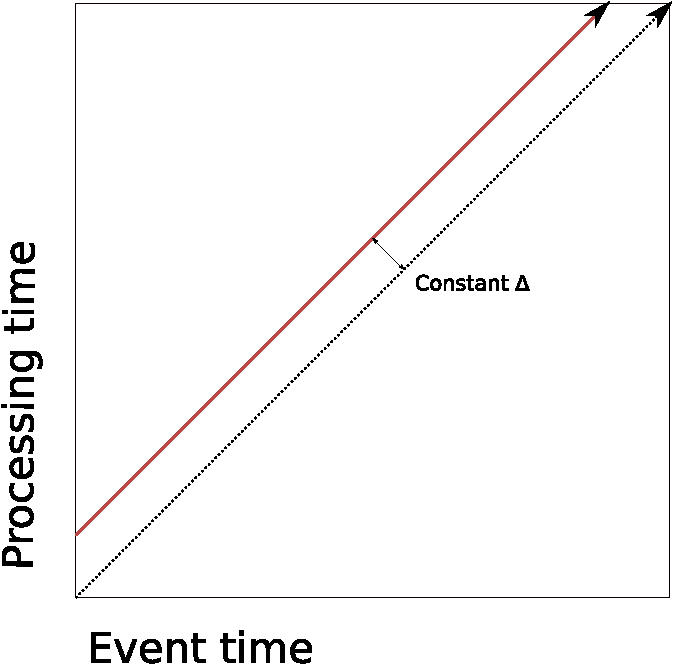
\includegraphics[width=0.8\linewidth]{constantskew.pdf}
  \caption{Constant time skew}
  \label{fig:constantskew}
\end{subfigure}%
\begin{subfigure}{.5\textwidth}
  \centering
  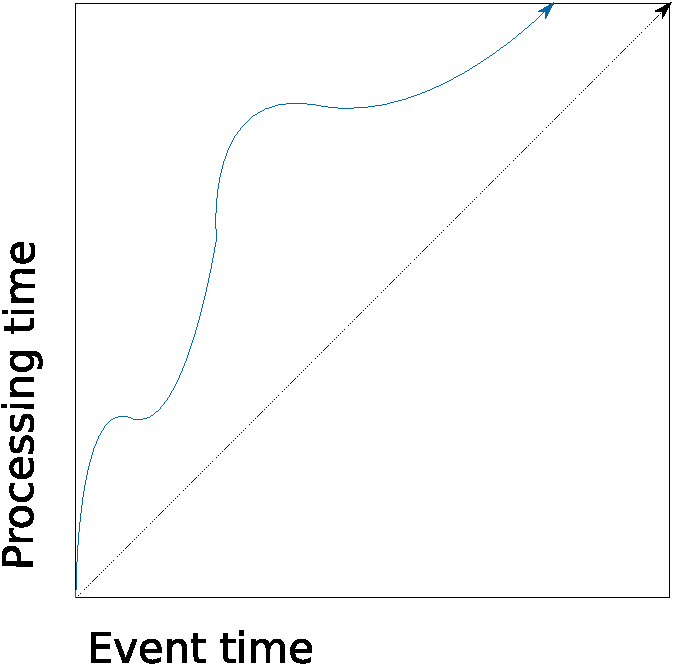
\includegraphics[width=.8\linewidth]{realskew.pdf}
  \caption{Irregular time skew}
  \label{fig:randomskew}
\end{subfigure}
\caption{Differences between ideal event time-process time skew and real world skew}
\label{fig:skew}
\end{figure}

Fixed timers are triggered based on system wall clocks, meaning that they do not
take into account event time. These timers are implemented using akka scheduler,
a system that allows scheduling message delivery between actors. They are a good
fit for computations that need to emit results at constant rate and do not need
a correlation with event times. However, there are occasions where it is needed
to know if events up to certain point in time have been processed. Due to the
nature of distributed systems it is difficult to know if at a given point in time,
all the events up to then have been received. In the ideal world, the
difference between event time and processing time would be a constant $\delta$ as
shown in figure~\ref{fig:constantskew}. Sadly, reality looks more
like figure~\ref{fig:randomskew}. Alcaudon tries to deal with this constraints
providing the grounds to work with and reason about out of order data. The choosen tool
is watermark timers, defined as follows:

\begin{definition}{Watermark}
Given a computation, $A$, let the oldest processed record in $A$ be a timestamp
corresponding to the oldest unfinished record in $A$.
Given this, watermark of $A$ is:
$min(oldest record of A, watermark of C : A depends on C)$
\end{definition}

Watermarks try to predict a timestamp $T_n$ signaling that up to that instant
all records have been received. Alcaudon implements a simple heuristic in order
to predict low watermarks. However more advanced techniques such us machine learning
can be used in order to predict low watermarks better. It is worth mentioning that this
very same algorithm was implemented by Google\cite{millwheel} and just about $0.001\%$
of records were dropped due to an incorrect prediction.
Therefore, using watermarks it is possible to configure timers that are
triggered once the watermark has reached a certain point, i.e. all records up to a
timestamp $T$ have been processed. 

In order to implement watermarks in Alcaudon, a system to replicate low
watermarks between different computations and streams is needed. One possible
option could be centralizing this knowledge in the cluster coordinator. The main
downside of this approach is that it could be a single-point of failure. Another
reason to avoid centralization is that watermarks are calculated in computation
basis, thus computations only need to have knowledge about their dependencies.
With this set of constraints \acs{CRDT}s are a good fit for the problem. They
are able to replicate changes among peers, they do not need coordination and
they provide eventual strong consistency. Again, akka provides an extension that
allows working with \acs{CRDT}s; akka distributed data. By default, this
extension provides different data type implementations such as counters, sets,
maps or registers. None of them are suitable to work with timestamps as is the
case of watermarks. Alcaudon implements a new \acs{CRDT} data type
\lstinline{GWatermark} that is able to satisfy the timestamps semantics as well
as \acs{CRDT} properties such as a monotonic merge function.
In Alcaudon, each \lstinline[columns=fixed]{ComputationExecutor} has a companion
actor, \lstinline[columns=fixed]{TimeExecutor}, who is in charge of keeping track
and triggering timers. This actor subscribes to \acs{CRDT} watermark changes that are
originated in computation dependencies(~\ref{code:timeExecutor}).

\begin{lstlisting}[language=scala, frame=trBL, label=code:timeExecutor, float=ht, caption = {TimerExecutor \acs{CRDT}s dependencies subscription}]
class TimerExecutor(computationId: String,
                    sources: Set[String],
                    initialWatermark: Long)
    extends Actor
    with ActorLogging {

      ...
  override def preStart(): Unit = {
    sources.foreach { srcId =>
      val key = GWatermarkKey(s"watermark-$srcId")
      replicator ! Subscribe(key, self)
      replicator ! Get(key, ReadMajority(2.seconds))
    }
  }
  ...
}
\end{lstlisting}

Once values from dependencies are known, the algorithm implementation to
calculate computation watermarks is straightforward(~\ref{code:watermarkUpdate}).

\begin{lstlisting}[language=scala, frame=trBL, label=code:watermarkUpdate, float=ht, caption = {Watermark update logic}]
def updateWatermarks(watermarkTimers: List[WatermarkTracker],
                     sourceWatermarks: Map[SourceID, Long],
                     timestamp: Long): Unit = {
  val minWatermarkSource =
    Try(sourceWatermarks.values.min).getOrElse(Long.MaxValue)
  latestWatermark = oldestComputationTimestamp.min(minWatermarkSource)
  val overdueTimers =
    watermarkTimers.filter(tracker => tracker.overdue(latestWatermark))
  val pendingTimers =
    watermarkTimers.filterNot(tracker => tracker.overdue(latestWatermark))
  val trackers = overdueTimers.map { tracker =>
    tracker.origin ! ExecuteTimer(tracker.timer)
    tracker.copy(lastWatermark = latestWatermark)
  } ::: pendingTimers
  context.become(working(trackers, sourceWatermarks))
}
\end{lstlisting}

Once watermarks are calculated, it is checked against the created timers if some
of them are past that point. If this is the case, a timer is
triggered(~\ref{code:watermarkUpdate}).

\subsection{Streams}

\begin{lstlisting}[language=scala, frame=trBL, label=code:recordstorage, float=ht, caption = {Stream record storage}]
case record: RawRecord =>
  val origin = sender()
  persist(RawStreamRecord(state.nextRecordSeq, record)) { event =>
    state.update(event)
    origin ! ReceiveACK(event.rawRecord.id)
    signalSubscribers(overwhelmedSubscribers)
    if (shouldTakeSnapshot)
      saveSnapshot(state)
\end{lstlisting}

In Alcaudon, streams represent the delivery instrument between different
computations. Computations subscribe to one or more streams and publish to zero
or more streams. As with computations, durability is a key part of streams,
meaning that during failure scenarios data published into a stream should be
recovered once the system is restarted. Streams are implemented as actors, and in
order to make them durable akka persistence has been used. As explained before,
with akka persistence it is possible to to store actor state. Alcaudon's streams
work largely as an append-only log, where computations or sources publish records
and they are delivered to subscribed computations. Each received record is
stored into a durable storage, in this case Cassandra. Internally, this
operation is done in batches, minimizing I/O overhead. This process is listed
in~\ref{code:recordstorage}. As it can be observed, stream publishers are
acknowledged when a record has been received. Again at least-once delivery
semantics are used to avoid any data loss. Once a record has been received,
pending records are sent to subscribers. A typical problem when implementing
publisher-subscriber systems is how to deal with slow-consumers. This is known as
flow control, and some patterns to solve this problem are listed below: 

\begin{itemize}
\item \textit{Back-pressure}: Consumers signal producers that they are able to
  process messages, defining message rate.
\item \textit{Managed queue pattern}: Where the consumer uses a bounded queue in
  order to store pending records.
\item \textit{Drop messages}: This pattern is an evolution of managed queue pattern. When
  the rate difference between producer and consumer is too big, messages are dropped.
  This pattern is biased towards system stability over correctness.
\item \textit{Throttling}: Throttle publisher output rate according to contracts
  with consumers.
\end{itemize}

Alcaudon deals with this problem using a hybrid approach. Stream actors store
the latest message offset acknowledged by each consumer. With this information, it
is possible to know an approximate consume rate for each consumer. A consumer is
considered overwhelmed when it has $n$ pending records to acknowledge, where $n$
is a configurable parameter. In order to avoid consumers instability, Alcaudon
streams stop sending messages to overwhelmed consumers for a while. To check if
consumers are able to handle new messages again, streams send them a record to
check if they are able to process it.They are taken out of quarantine if they
are able to handle it. This process is represented as a sequence diagram in
figure~\ref{fig:flowcontrol}.

\begin{figure}[!h]
  \centering
  \scalebox{0.5}{
    \input{figures/flowcontrol.latex}
  }
\caption{Alcaudon flow control sequence diagram}
\label{fig:flowcontrol}
\end{figure}

As described in previous sections, users should provide a key extraction
function. With this function, each record gets a key assigned. This allows to
parallelize computations using that key as a routing property. In particular,
Alcaudon uses consistent hashing in order to decide to which computation
executor a record should be delivered~\ref{fig:streamkeypart}. The number of
parallel computations is configurable as a global parameter in Alcaudon
settings.

\begin{figure}
  \centering
  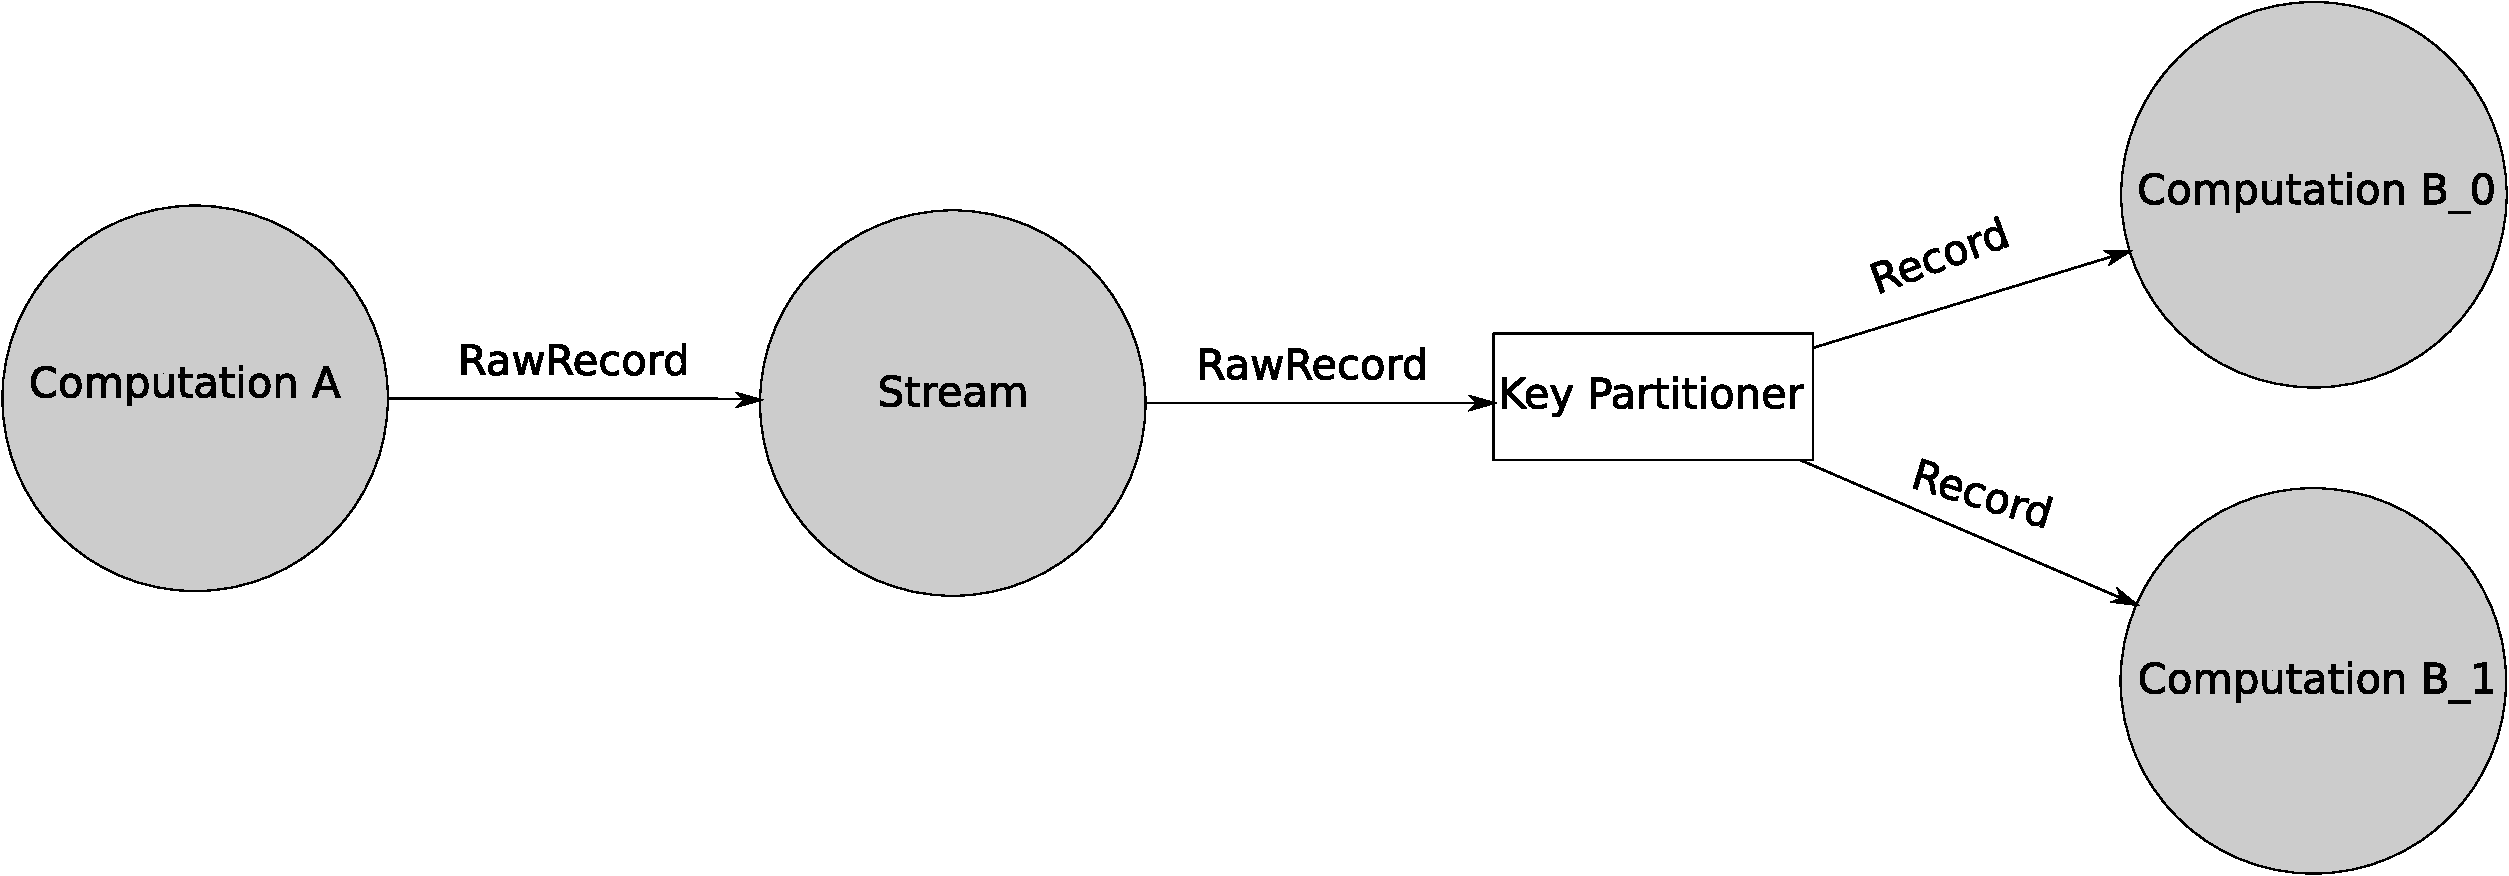
\includegraphics[width=0.8\textwidth]{stream.pdf}
  \caption{Streams key partitioning}
  \label{fig:streamkeypart}
\end{figure}

\section{Coordinator node}

Finally, coordinator node architecture design will be presented. This component
is in charge of keeping track of computation nodes, gathering different metrics,
creating new dataflow pipelines and scheduling them. A high level overview of this
system can be found in figure~\ref{fig:coordinatormodules}.

\begin{figure}[!h]
  \centering
  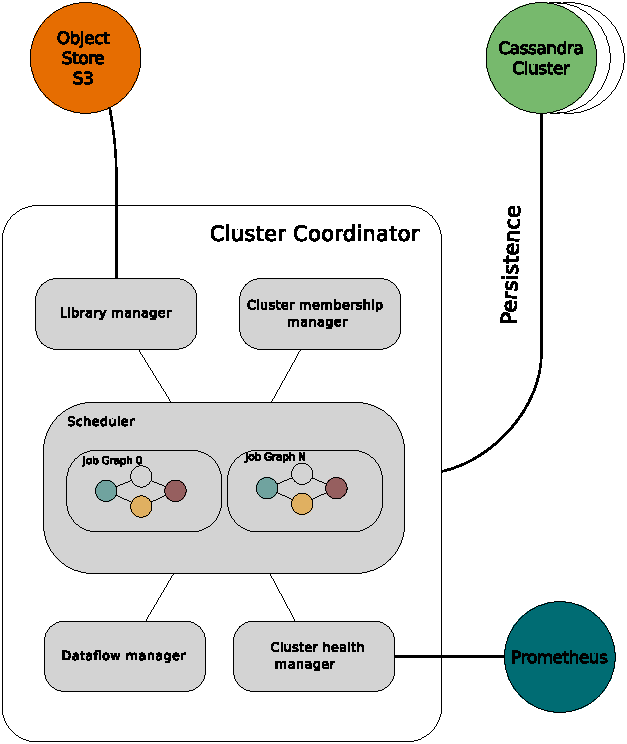
\includegraphics[width=0.6\textwidth]{coordinator.pdf}
  \caption{Coordinator node modules}
  \label{fig:coordinatormodules}
\end{figure}

Alcaudon coordinator node is composed of modules defined below:
\begin{itemize}
  \item \textit{Library manager}: It is in charge of storing user defined code
    into an object storage service.
  \item \textit{Cluster membership manager}: Module that manages the life-cycle of
    computing nodes in order to be able to schedule tasks in them.
  \item \textit{Dataflow manager}: Dataflow manager is the interface between
    users and the cluster. It defines how users create, monitor or destroy
    dataflow pipelines.
  \item \textit{Scheduler}: Scheduler is in charge of, given a dataflow pipeline
    to be deployed, get a deployment plan as optimal as possible.
  \item \textit{Cluster health manager}: This module is in charge of collecting
    different metrics such as CPU usage, memory usage, number of records
    processed, unhealthy nodes, etc. This nodes exposes an \acs{HTTP} interface
    so Prometheus is able to pull metrics data from it. It is used in
    combination with Grafana, a tool to generate time series dashboards.
\end{itemize}

Modules such as Library Manager and Dataflow Manager have been exposed in
previous sections, therefore this section will be focused on scheduling, cluster
membership manager, cluster health manager.

\subsection{Scheduler}

\begin{figure}[!h]
  \centering
  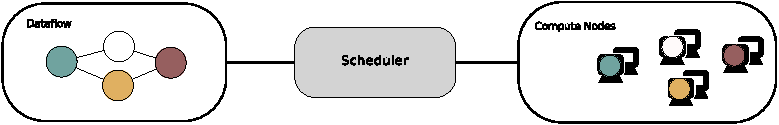
\includegraphics[width=0.8\textwidth]{scheduling.pdf}
  \caption{Scheduling process}
  \label{fig:scheduler}
\end{figure}

When dataflow pipelines are created, Alcaudon should deploy these computations
into available compute nodes~\ref{fig:scheduler}. Some desirable properties that
these deployments should have are:

\begin{itemize}
\item High cluster utilization
\item Fast job completion
\item Fairness
\item Efficiency
\end{itemize}

As it was described in previous sections, this problem is know as
\textit{flexible Job-shop scheduling problem} and it is cataloged as a NP-Hard
problem. Existing algorithms are based on heuristics and usually these
algorithms are biased towards fairness, performance or efficiency.
Alcaudon uses an state of the art cluster scheduler platform\cite{firmament},
named Firmament. It allows to use \acf{HTTP} in order to perform scheduling
requests. An interesting feature that this scheduler offers is that it allows
using different scheduling policies. These policies are listed below.

\begin{itemize}
\item \textit{Trivial}: Fixed costs, tasks always schedule if resources are idle.
\item \textit{Random}: Random costs, for fuzz tests.
\item \textit{SJF}: Shortest job first policy based on avg. past runtimes.
\item \textit{Quincy}: Original Quincy cost model, with data locality.       
\item \textit{Whare}: Implementation of Whare-Map's M and MCs policies.
\item \textit{Coco}: Coordinated co-location model.
\item \textit{Octopus}: Simple load balancing based on task counts.     
\item \textit{Void}: Bogus cost model used for KB with simple scheduler.  
\item \textit{NET-BW}: Network-bandwidth-aware cost model (avoids hotspots).  
\end{itemize}

After performing tests with different scheduling policies, Alcaudon uses
\textit{CoCo} scheduling policy as the defualt scheduling policy. It is
preferred to co-locate computations in order to save network round-trips.
However, it is possible to configure Alcaudon to use different policies.
Firmament calculations could take a long time, depending on the complexity
and \acs{DAG} to schedule size. In order to avoid long blocking \acs{HTTP}
requests, when a new scheduling request is performed, an operation code
is returned. With this code is possible to inspect how the operation is
evolving and eventually get a result. This process is summarized as as
sequence diagram in figure~\ref{fig:schedulefirmament}.

\begin{figure}[!h]
  \centering
  \scalebox{0.5}{
    \input{figures/schedulefirmament.latex}
  }
\caption{Sequence diagram for interaction between Firmament and Alcaudon}
\label{fig:schedulefirmament}
\end{figure}


\subsection{Cluster health manager}

Operating large distributed systems is challenging. In these environments,
multiple components are working together and eventually some of them could fail.
If the available tools to debug and monitor them are not adequate, finding a
problematic component could take hours. Given these facts, providing the tools
to monitor distributed systems is mandatory. One of Alcaudon's aims is to
provide metrics and mechanisms to deal with this problem. In order to implement
this feature, Prometheus has been used as a time series database and Grafana
as the dashboards generator. 

The component in charge of collecting metrics is \textit{cluster health
  manager}. This component listens to akka cluster events, in order to determine
the health from different nodes in the system. In also listens to some statistics
regarding actors, such as number of messages sent, mailbox size, CPU usage,
memory usage, statistics about jvm fork join pool,
etc (\ref{code:metricsSample}). All these metrics are stored into Prometheus,
allowing to query that times series data efficiently. Finally, Grafana consumes
data from Prometheus in order to plot different metrics.

\begin{lstlisting}[language=scala, frame=trBL, label=code:metricsSample, float=ht, caption = {Example of Alcaudon exposed metrics}]
# HELP akka_dispatcher_forkjoinpool_steal_count Akka ForkJoinPool Dispatcher Steal Count
# TYPE akka_dispatcher_forkjoinpool_steal_count gauge
akka_dispatcher_forkjoinpool_steal_count{dispatcherName="WebServer_akka.actor.default-dispatcher",} 49.0
# HELP akka_actor_group_processing_time Akka Actor Group processing time (Nanos)
# TYPE akka_actor_group_processing_time counter
akka_actor_group_processing_time{groupName="all",} 1.04116122E8
# HELP akka_router_processing_time_webserver_system_io_tcp_selectors Akka Router processing time (Nanos)
# TYPE akka_router_processing_time_webserver_system_io_tcp_selectors counter
akka_router_processing_time_webserver_system_io_tcp_selectors 2.541922E7
# HELP akka_router_error_count_webserver_system_io_tcp_selectors Akka Router errors
# TYPE akka_router_error_count_webserver_system_io_tcp_selectors counter
akka_router_error_count_webserver_system_io_tcp_selectors 0.0
# HELP akka_actor_group_mailboxes_size Akka Actor Group mailboxes size
# TYPE akka_actor_group_mailboxes_size gauge
akka_actor_group_mailboxes_size{groupName="all",} 1.0
\end{lstlisting}

Grafana~\ref{fig:grafana} allows to define custom dashboards and configure
alerts. Alerting is essential when monitoring distributed system. It is possible
to define alerts based on predictive models and warn system operators before
the actual problem occurs, i.e. using simple linear regression for disk
size. An example for Alcaudon's domain could be, based on the growth of pending
dataflow pipelines to schedule, trigger an alert if that metric keeps growing for
2 hours, meaning that the number of compute nodes is not enough.

\begin{figure}[!h]
\begin{center}
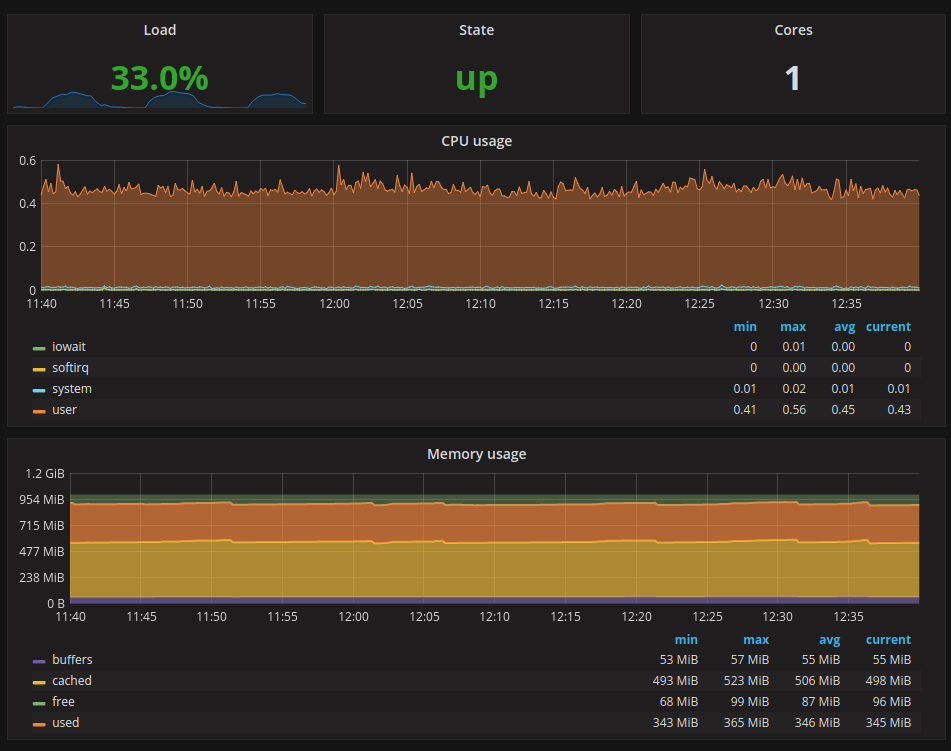
\includegraphics[width=0.7\textwidth]{grafana.png}
\caption{Grafana dasboard}
\label{fig:grafana}
\end{center}
\end{figure}

\section{Alcaudon deployment}

In order to deploy the different components of Alcaudon, they are distributed as
docker containers. Latest Alcaudon versions are available in
docker-hub\footnote{https://hub.docker.com/u/fcofdezc/}. Using containers to
deploy Alcaudon, abstracts away all the build process details creating a
reproducible environment to execute it. Furthermore, containers have become an
industry de facto standard to deliver software. Distributing Alcaudon as Docker
containers makes it suitable to be deployed using container schedulers such as
Kubernets, Mesos or AWS ECS, leveraging all the deployment complexities to
those tools.

In order to deploy a cluster coordinator:

\begin{lstlisting}
  $ docker run --volume /etc/alcaudon/alcaudon.conf:/etc/alcaudon/alcaudon.conf fcofdezc/alcaudon-coordinator
\end{lstlisting}

In order to deploy compute nodes:

\begin{lstlisting}
  $ docker run --volume /etc/alcaudon/alcaudon-compute.conf:/etc/alcaudon/alcaudon-compute.conf fcofdezc/alcaudon-compute
\end{lstlisting}

Alcaudon library is published into Sonatype repository. In order to include it into
an SBT build and start building Alcaudon Dataflow pipelines, this dependency should be added:

\begin{lstlisting}
resolvers += 
  "Sonatype OSS Snapshots" at "https://oss.sonatype.org/content/repositories/snapshots"
libraryDependencies += "com.github.fcofdez" % "alcaudon"
\end{lstlisting}

\chapter{Results}

In this chapter, attained results during the development of this project will be
presented. First, a series of benchmarks have been used in order to exercise key
Alcaudon modules and measure how the system behaves. Then, a possible real
application for Alcaudon will be stated. To conclude, a summary of accomplished
objectives is presented.

\section{Benchmarks}

Alcaudon has been tested thoroughly, both using traditional testing techniques
as well as more state-of-the-art techniques such as property based testing.
These tests can guarantee correctness in terms of behavior, but they do not
measure system precision in terms of performance goals. Even though Alcaudon
has been designed carefully, using the adequate data structures and taking
care of performance, empiric results are needed. It is known that creating
accurate benchmarks is complex~\cite{benchbias}, as there are many factors
that can lead to misleading results. Presented benchmarks are implemented using
JMH\footnote{http://openjdk.java.net/projects/code-tools/jmh/}.

\subsection{Computation execution benchmark}

This benchmark measures the number of computations per second that Alcaundon can
handle.

\begin{lstlisting}
# JMH version: 1.19
# VM version: JDK 1.8.0_131, VM 25.131-b11
# VM invoker: /usr/lib/jvm/java-8-oracle/jre/bin/java
# VM options: <none>
# Warmup: 15 iterations, 1 s each
# Measurement: 15 iterations, 1 s each
# Timeout: 10 min per iteration
# Threads: 1 thread, will synchronize iterations
# Benchmark mode: Throughput, ops/time
# Benchmark: org.alcaudon.runtime.ComputationBenchmark.throughput

# Fork: 1 of 1
# Warmup Iteration   1: 2838.544 ops/s
# Warmup Iteration   2: 12645.095 ops/s
# Warmup Iteration   3: 13336.237 ops/s
# Warmup Iteration   4: 15380.058 ops/s
# Warmup Iteration   5: 16003.125 ops/s
# Warmup Iteration   6: 15388.756 ops/s
# Warmup Iteration   7: 14816.361 ops/s
# Warmup Iteration   8: 14820.269 ops/s
# Warmup Iteration   9: 14826.327 ops/s
# Warmup Iteration  10: 15995.409 ops/s
# Warmup Iteration  11: 17395.065 ops/s
# Warmup Iteration  12: 17396.909 ops/s
# Warmup Iteration  13: 16674.274 ops/s
# Warmup Iteration  14: 16668.055 ops/s
# Warmup Iteration  15: 16668.801 ops/s
Iteration   1: 16006.082 ops/s
Iteration   2: 16021.392 ops/s
Iteration   3: 16002.350 ops/s
Iteration   4: 16673.828 ops/s
Iteration   5: 16002.128 ops/s
Iteration   6: 13795.418 ops/s
Iteration   7: 14293.416 ops/s
Iteration   8: 12902.619 ops/s
Iteration   9: 14826.131 ops/s
Iteration  10: 14279.800 ops/s
Iteration  11: 14834.078 ops/s
Iteration  12: 13347.936 ops/s
Iteration  13: 14818.898 ops/s
Iteration  14: 14811.602 ops/s
Iteration  15: 14286.494 ops/s


Result "org.alcaudon.runtime.ComputationBenchmark.throughput":
  14860.145 +-(99.9%) 1171.277 ops/s [Average]
  (min, avg, max) = (12902.619, 14860.145, 16673.828), stdev = 1095.613
  CI (99.9%): [13688.868, 16031.422] (assumes normal distribution)
\end{lstlisting}

\subsection{Stream benchmark}

This benchmark measures the number of records that a stream can handle using
the network stack.

\begin{lstlisting}
# JMH version: 1.19
# VM version: JDK 1.8.0_131, VM 25.131-b11
# VM invoker: /usr/lib/jvm/java-8-oracle/jre/bin/java
# VM options: <none>
# Warmup: 15 iterations, 1 s each
# Measurement: 15 iterations, 1 s each
# Timeout: 10 min per iteration
# Threads: 1 thread, will synchronize iterations
# Benchmark mode: Throughput, ops/time
# Benchmark: org.alcaudon.runtime.StreamBenchmark.throughput

# Fork: 1 of 1
# Warmup Iteration   1: 9321.185 ops/s
# Warmup Iteration   2: 31098.503 ops/s
# Warmup Iteration   3: 56383.813 ops/s
# Warmup Iteration   4: 89775.005 ops/s
# Warmup Iteration   5: 92496.201 ops/s
# Warmup Iteration   6: 66532.817 ops/s
# Warmup Iteration   7: 56076.426 ops/s
# Warmup Iteration   8: 63003.972 ops/s
# Warmup Iteration   9: 59410.283 ops/s
# Warmup Iteration  10: 58177.190 ops/s
# Warmup Iteration  11: 59273.481 ops/s
# Warmup Iteration  12: 61445.394 ops/s
# Warmup Iteration  13: 52879.995 ops/s
# Warmup Iteration  14: 57380.524 ops/s
# Warmup Iteration  15: 46046.720 ops/s
Iteration   1: 69487.193 ops/s
Iteration   2: 28153.126 ops/s
Iteration   3: 65117.851 ops/s
Iteration   4: 51256.389 ops/s
Iteration   5: 44682.554 ops/s
Iteration   6: 43606.471 ops/s
Iteration   7: 31458.501 ops/s
Iteration   8: 66222.260 ops/s
Iteration   9: 61828.791 ops/s
Iteration  10: 24873.576 ops/s
Iteration  11: 58282.826 ops/s
Iteration  12: 61180.519 ops/s
Iteration  13: 12427.225 ops/s
Iteration  14: 55291.714 ops/s
Iteration  15: 38296.842 ops/s

Result "org.alcaudon.runtime.StreamBenchmark.throughput":
  47477.722 +-(99.9%) 18537.348 ops/s [Average]
  (min, avg, max) = (12427.225, 47477.722, 69487.193), stdev = 17339.847
  CI (99.9%): [28940.375, 66015.070] (assumes normal distribution)
\end{lstlisting}

\subsection{Record router benchmark}

This benchmark measures the number of records that a router can route.

\begin{lstlisting}
# JMH version: 1.19
# VM version: JDK 1.8.0_131, VM 25.131-b11
# VM invoker: /usr/lib/jvm/java-8-oracle/jre/bin/java
# VM options: <none>
# Warmup: 15 iterations, single-shot each
# Measurement: 15 iterations, single-shot each
# Timeout: 10 min per iteration
# Threads: 1 thread
# Benchmark mode: Single shot invocation time
# Benchmark: org.alcaudon.KeyRouterBenchmark.timePerRoute

# Fork: 1 of 1
# Warmup Iteration   1: 381472.618 us/op
# Warmup Iteration   2: 150042.661 us/op
# Warmup Iteration   3: 176778.359 us/op
# Warmup Iteration   4: 106955.031 us/op
# Warmup Iteration   5: 99704.939 us/op
# Warmup Iteration   6: 57248.973 us/op
# Warmup Iteration   7: 37281.762 us/op
# Warmup Iteration   8: 85989.580 us/op
# Warmup Iteration   9: 23317.259 us/op
# Warmup Iteration  10: 33628.435 us/op
# Warmup Iteration  11: 23899.475 us/op
# Warmup Iteration  12: 22373.551 us/op
# Warmup Iteration  13: 22630.460 us/op
# Warmup Iteration  14: 22016.820 us/op
# Warmup Iteration  15: 21163.906 us/op
Iteration   1: 23386.227 us/op
Iteration   2: 26890.087 us/op
Iteration   3: 27592.136 us/op
Iteration   4: 25660.356 us/op
Iteration   5: 26705.218 us/op
Iteration   6: 49419.625 us/op
Iteration   7: 54298.073 us/op
Iteration   8: 116075.003 us/op
Iteration   9: 28676.928 us/op
Iteration  10: 19761.540 us/op
Iteration  11: 19466.265 us/op
Iteration  12: 23165.587 us/op
Iteration  13: 18574.349 us/op
Iteration  14: 21910.841 us/op
Iteration  15: 20325.704 us/op


Result "org.alcaudon.KeyRouterBenchmark.timePerRoute":
  N = 15
  mean =  33460.529 +-(99.9%) 26862.874 us/op

  Histogram, us/op:
    [ 10000.000,  20000.000) = 3
    [ 20000.000,  30000.000) = 9
    [ 30000.000,  40000.000) = 0
    [ 40000.000,  50000.000) = 1
    [ 50000.000,  60000.000) = 1
    [ 60000.000,  70000.000) = 0
    [ 70000.000,  80000.000) = 0
    [ 80000.000,  90000.000) = 0
    [ 90000.000, 100000.000) = 0
    [100000.000, 110000.000) = 0

  Percentiles, us/op:
      p(0.0000) =  18574.349 us/op
     p(50.0000) =  25660.356 us/op
     p(90.0000) =  79008.845 us/op
     p(95.0000) = 116075.003 us/op
     p(99.0000) = 116075.003 us/op
     p(99.9000) = 116075.003 us/op
     p(99.9900) = 116075.003 us/op
     p(99.9990) = 116075.003 us/op
     p(99.9999) = 116075.003 us/op
    p(100.0000) = 116075.003 us/op
\end{lstlisting}

\section{Alcaudon application}

Once Alcaudon has been described in detail, its full potential can be unveiled
in a real world scenario. For this example, a
public\footnote{http://www.nyc.gov/html/tlc} data set of the New York City Taxi
and Limousine Commission (TLC) will be used. This data set contains records
about taxi trips in New York from different years. The goal of this example is
to use this data set as a real unbounded data source, where taxi customers take
taxis for a ride from point A to point B and this information is delivered into
Alcaudon. With this information it is possible to build an Alcaudon dataflow
topology in order to detect spikes in rides to certain parts of the city, for
example during a concert. For companies like Uber, where prices fluctuate
depending on demand, processing this information in \textit{real time} is
fundamental. This example will build an Alcaudon dataflow topology in order to
aggregate rides per zone and emit results in constant time windows. These
aggregated results will be published into ElasticSearch to be visualized later
on as shown in figure~\ref{fig:rides}. Business stakeholders can use these
dashboards in order to take decisions with the latest information available.

\begin{figure}[!h]
\begin{center}
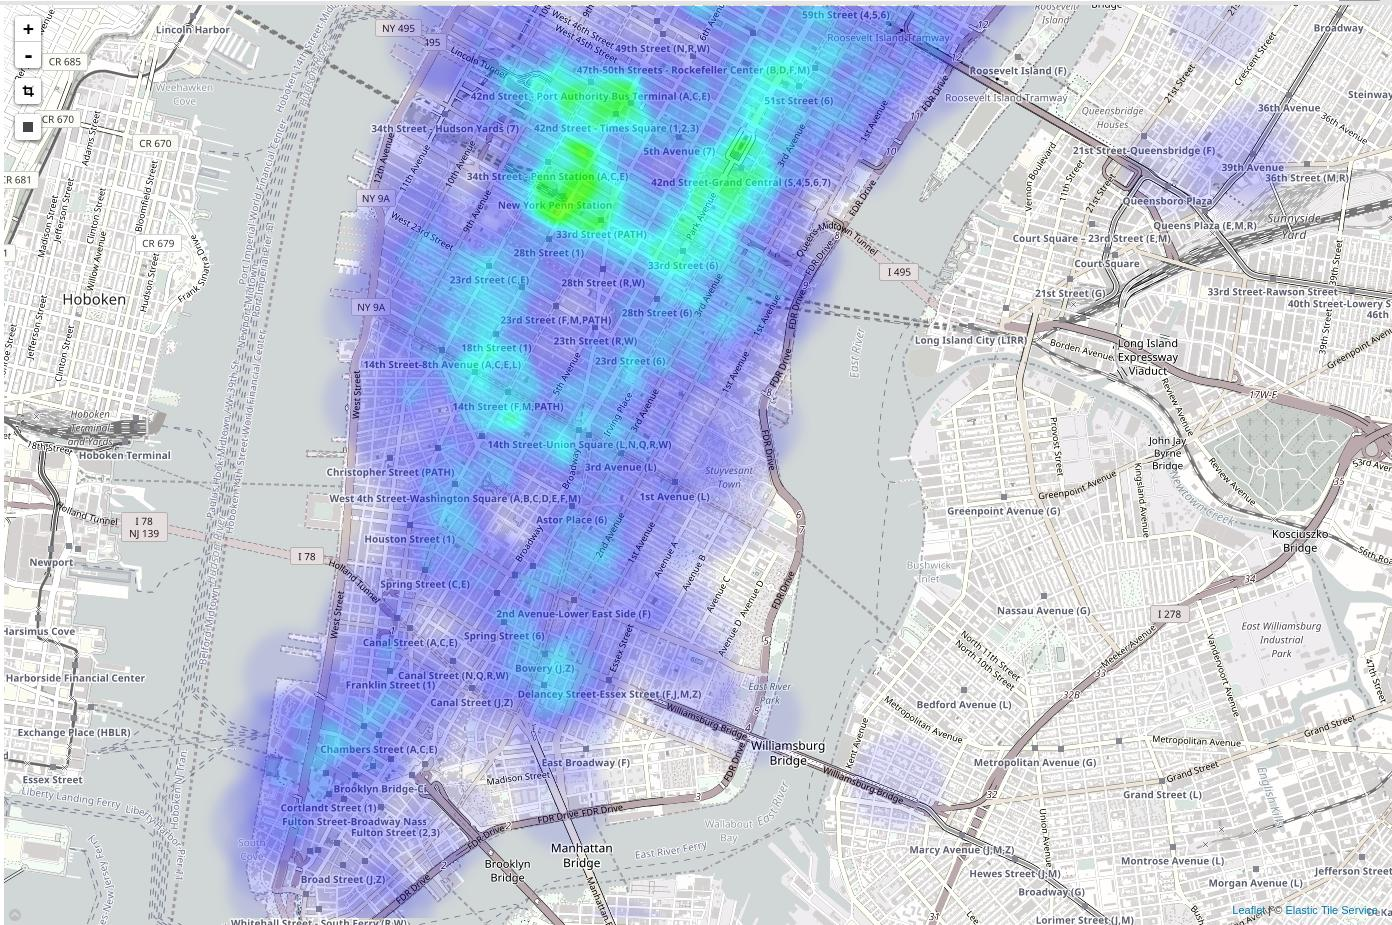
\includegraphics[width=0.8\textwidth]{nyrides.jpg}
\caption{Example dashboard}
\label{fig:rides}
\end{center}
\end{figure}

Since this is a synthetic example, a custom source has been defined in order to
emit ride events using their original timestamps. Ride information contains
different fields, but for the purposes of this example, a simple representation
has been created, listed in~\ref{code:ride}. In order to aggregate location
information, the map is divided into cells, where each ride belongs to one of
these cells. This subdivision in cells is used in order to define a key per
record as it can be found in listing~\ref{code:keyExtractorNY}.

The main goal of this example is to publish updated data about the number of
passengers taking rides in different places of the city, to later on visualize
this data in a dashboard. First of all, rides that are not taking place in New
York are filtered out~(\ref{code:computationFilterRide}) and published into a new
stream. These filtered rides are consumed by
RidePassengerCountComputation~\ref{code:computationRide} that is responsible
for keeping track of the number of passengers per cell and updating them when new rides
arrive into the system. A timer is set-up, when this timer is triggered, the
information stored up to that point, in this case the number of ride passengers
per cell, is published into a Sink. In addition to counting the number of
passengers, this computation publishes into a different sink when the number of
passengers arriving into a specific cell is bigger than a setting. This is
useful when alerts for different events are needed. Dataflow topology definition
can be found in listing~\ref{code:rideDataflow}. This example shows the
potential of unbounded data-set processing, and the strengths of Alcaudon in
particular.

\begin{lstlisting}[language=scala, frame=trBL, label=code:ride, float=ht, caption = {Ride \acs{ADT}}]
case class Ride(id: Long, time: DateTime, location: Point, passengerCount: Int)
\end{lstlisting}

\begin{lstlisting}[language=scala, frame=trBL, label=code:computationFilterRide, float=ht, caption = {Computation to filter out non New York rides}]
class FilterRideComputation extends Computation {
  def processRecord(record: Record): Unit = {
    val ride: Ride = deserialize(record.value)
    if (ride.isInNYC())
      produceRecord(nycRides, record)
  }

  def processTimer(timeStamp: Timer): Unit = {}
}
\end{lstlisting}

\begin{lstlisting}[language=scala, frame=trBL, label=code:keyExtractorNY, float=ht, caption = {Key extractor function}]
class RideKeyExtractor extends KeyExtractor {
  def extractKey(msg: Array[Byte]): String = {
    val ride: Ride = deserialize(msg)
    Utils.locationToCell(ride.location)
  }
}
\end{lstlisting}

\begin{lstlisting}[language=scala, frame=trBL, label=code:computationRide, float=ht, caption = {Ride \acs{ADT}}]
class RidePassengerCountComputation extends Computation {
  def processRecord(record: Record): Unit = {
    val ride: Ride = deserialize(record.value)
    val count: Int = get(record.key) + ride.passengerCount
    if (count > settings.alertPassengers)
      produceRecord(alertSink, RawRecord(serialize(record.key), record.timestamp))
    set(count + ride.passengerCount)
    setTimer(FixedRecurrentTimer(cell, 5.minutes))
  }

  def processTimer(timeStamp: Timer): Unit = {
    val location = Utils.cellToLocation(timer.tag)
    val totalPassengerCount = get(timer.tag)
    produceRecord(elasticSink, RawRecord(serialize((location, totalPassengerCount)), record.timestamp))
  }
}
\end{lstlisting}

\begin{lstlisting}[language=scala, frame=trBL, label=code:rideDataflow, float=ht, caption = {Ride dataflow creation}]
val dataflow = DataflowBuilder("ridesCounter")
  .withSource("taxiRides", TaxiRides())
  .withComputation("filterNYRides",
    FilterRideComputation,
    OutputStreams("nycRides"),
    AlcaudonInputStream("taxiRides")
  .withComputation("passengerCount",
    RidePassengerCountComputation,
    OutputStreams("elasticSink", "alertSink"),
    AlcaudonInputStream("nycRides", new RideKeyExtractor())
  .withSink("elasticSink", ElasticSearchSink)
  .withSink("alertSink", HTTPSink(settings.alertEndpoint))
  .build()
\end{lstlisting}

\section{Accomplished objectives}

During the development of this project, all objectives defined at the beginning
of this document have been accomplished. Alcaudon provides all the necessary
tools to deploy distributed stream data processing pipelines. It attains this
objective by supplying an abstract model, the Computation \acs{API}, that users
implement, leveraging the all the complexities around fault-tolerant distributed
models to Alcaudon.

Regarding specific objectives, these have been accomplished as well:
%
\begin{itemize}
\item Alcaudon provides an abstraction in order to create distributed
  computations; computation \acs{API} alongside the dataflow builder.
\item The system provides exactly-once processing semantics, using at-least once
  delivery in combination with idempotent record processing. In order to achieve
  idempotence, state-of-the-art probabilistic data structures have been used as
  well as persistent actors to guarantee persistent state durability.
\item The system provides watermark based timers in order to work with
  out-of-order data. The implementation of this subsystem uses state-of-the-art
  coordination-free distributed data types in order to replicate knowledge about
  time event evolution inside the system.
\item Dataflow \acs{DAG}s are scheduled into available compute nodes using an
  state-of-the-art flexible cluster scheduler~\cite{firmament}. Different scheduling
  policies can be configured depending on the needs, where the default choice is
  biased towards co-location.
\item Several sources and sinks are provided by default such as Twitter streaming
  API, TCP Sockets or Apache Kafka. However it is possible to implement new ones
  just extending SourceFn and SinkFN interfaces.
\item Alcaudon provides an elastic distributed implementation where compute
  nodes can join the cluster in the events of burst of load. The system has been
  designed in order to be resilient and fault-tolerant. The actor model has
  facilitated the development in terms of resilience due to is supervision mechanism that
  allows to isolate failure.
\item Alcaudon provides different metrics about the state of the system. It has been
  integrated with industry proven technologies in the space of monitoring such as
  Prometheus and Graphana. Using these tools it is possible to create a rich set
  of alerts and dashboards giving a good overview of how the different components
  of Alcaudon perform.
\item Alongside the previously presented results, Alcaudon is distributed using Docker
  containers and its library is available in SonaType repository. This makes almost
  trivial to deploy a full-featured Alcaudon cluster.
\end{itemize}

\section{Future work}

Given that Alcaudon has been designed in a modular way and it has many automatic
tests, including new features should be effortless. In this section some future work
that could be done to the platform is presented.

\begin{itemize}
\item Improve system performance avoiding object allocations in certain
  sensitive parts of the system such as the Streams. High allocation rate
  usually hurts managed systems performance due to garbage collection. Some
  systems such as Netty\footnote{https://netty.io/} use pre-allocated memory buffers
  in order to avoid heap allocations as much as possible. This approach could be
  explored in order to improve Alcaudon performance.
\item Implement a machine learning algorithm in order to select a scheduling policy
  based on similar already run dataflow pipelines, improving the overall performance.
\item Implement a fully functional programming interface on top of the
  computation API in order to offer a more expressive API to the users.
  Providing \textit{combinators} such as map, groupBy, filter, etc.
\item Alcaudon watermark algorithm is just a minimal version. Used heuristic
  could be improved and it would be interesting to test different machine
  learning algorithms in order to predict watermarks. Another interesting
  approach to the problem that watermarks solve is to use virtual tables as
  Apache Kafka Streaming does~\cite{kafkastreams}.
\end{itemize}


\appendix
\appendixtitle
\chapter{Alcaudon configuration}

\begin{lstlisting}
akka {
  loglevel = "INFO"
  stdout-loglevel = "INFO"

  persistence {
    journal.plugin = "cassandra-journal"
    snapshot-store.plugin = "cassandra-snapshot-store"
  }

  actor {

  provider = "akka.cluster.ClusterActorRefProvider"

    deployment {
      computation-dispatcher {
        fork-join-executor {
          parallelism-min = 8
          parallelism-factor = 3.0
          parallelism-max = 64
        }
        throughput = 50
      }
    }

    serializers {
      kryo = "com.romix.akka.serialization.kryo.KryoSerializer"
      gwatermark = "org.alcaudon.runtime.GWatermarkSerializer"
    }


    serialization-bindings {
      "org.alcaudon.core.RawStreamRecord" = kryo
      "org.alcaudon.core.AlcaudonStream$Subscribe" = kryo
      "org.alcaudon.core.AlcaudonStream$ACK" = kryo
      "org.alcaudon.core.StreamState" = kryo
      "org.alcaudon.core.State$SetValue" = kryo
      "org.alcaudon.core.State$SetTimer" = kryo
      "org.alcaudon.core.State$Transaction" = kryo
      "org.alcaudon.runtime.ComputationReifier$ComputationState" = kryo
      "org.alcaudon.runtime.GWatermark" = gwatermark
    }

    kryo  {
      type = "graph"
      idstrategy = "automatic"
      buffer-size = 4096
      max-buffer-size = -1
      use-manifests = true
      use-unsafe = false
      post-serialization-transformations = "off"
      implicit-registration-logging = true
      kryo-trace = false
      resolve-subclasses = true
    }
  }

  extensions = ["com.romix.akka.serialization.kryo.KryoSerializationExtension$"]

}

alcaudon {
  computation {
    timeout = 600s
    max-failures = 12
    cuckoo-filter-records = 100000
    snapshot-interval = 10000
    computing-slots = 8
    parallelism = 4
  }

  streams {
    flow-control {
      backoff-time = 10s
      overwhelmed-retry-time = 10s
      overwhelmed-delay = 100
    }
    snapshot-interval = 10000
  }

  scheduling-policy = "CoCo"
  consistency-constraint = "HIGH"


  blob {
    directory = "/tmp/alcaudon"
    download-timeout = 1h
    s3 {
      access-key = "access-key"
      secret-key = "access-secret"
      region = "us-east-1"
    }
  }
}
\end{lstlisting}

{\small \chapter{GNU Free Documentation License}
\vspace{1.5cm}

Version 1.3, 3 November 2008

Copyright © 2000, 2001, 2002, 2007, 2008 Free Software Foundation,
Inc. <\url{http://fsf.org/}>

Everyone is permitted to copy and distribute verbatim copies of this
license document, but changing it is not allowed.


\setcounter{section}{-1}

\titleformat{\section}
  {\normalfont\normalsize\bfseries}{\arabic{section}.}{1em}{}

\section{PREAMBLE}

The purpose of this License is to make a manual, textbook, or other
functional and useful document ``free'' in the sense of freedom: to
assure everyone the effective freedom to copy and redistribute it,
with or without modifying it, either commercially or
noncommercially. Secondarily, this License preserves for the author
and publisher a way to get credit for their work, while not being
considered responsible for modifications made by others.

This License is a kind of ``copyleft'', which means that derivative
works of the document must themselves be free in the same sense. It
complements the GNU General Public License, which is a copyleft
license designed for free software.

We have designed this License in order to use it for manuals for free
software, because free software needs free documentation: a free
program should come with manuals providing the same freedoms that the
software does. But this License is not limited to software manuals; it
can be used for any textual work, regardless of subject matter or
whether it is published as a printed book. We recommend this License
principally for works whose purpose is instruction or reference.


\section{APPLICABILITY AND DEFINITIONS}

This License applies to any manual or other work, in any medium, that
contains a notice placed by the copyright holder saying it can be
distributed under the terms of this License. Such a notice grants a
world-wide, royalty-free license, unlimited in duration, to use that
work under the conditions stated herein. The ``Document'', below, refers
to any such manual or work. Any member of the public is a licensee,
and is addressed as ``you''. You accept the license if you copy, modify
or distribute the work in a way requiring permission under copyright
law.

A ``Modified Version'' of the Document means any work containing the
Document or a portion of it, either copied verbatim, or with
modifications and/or translated into another language.

A ``Secondary Section'' is a named appendix or a front-matter section of
the Document that deals exclusively with the relationship of the
publishers or authors of the Document to the Document's overall
subject (or to related matters) and contains nothing that could fall
directly within that overall subject. (Thus, if the Document is in
part a textbook of mathematics, a Secondary Section may not explain
any mathematics.) The relationship could be a matter of historical
connection with the subject or with related matters, or of legal,
commercial, philosophical, ethical or political position regarding
them.

The ``Invariant Sections'' are certain Secondary Sections whose titles
are designated, as being those of Invariant Sections, in the notice
that says that the Document is released under this License. If a
section does not fit the above definition of Secondary then it is not
allowed to be designated as Invariant. The Document may contain zero
Invariant Sections. If the Document does not identify any Invariant
Sections then there are none.

The ``Cover Texts'' are certain short passages of text that are listed,
as Front-Cover Texts or Back-Cover Texts, in the notice that says that
the Document is released under this License. A Front-Cover Text may be
at most 5 words, and a Back-Cover Text may be at most 25 words.

A ``Transparent'' copy of the Document means a machine-readable copy,
represented in a format whose specification is available to the
general public, that is suitable for revising the document
straightforwardly with generic text editors or (for images composed of
pixels) generic paint programs or (for drawings) some widely available
drawing editor, and that is suitable for input to text formatters or
for automatic translation to a variety of formats suitable for input
to text formatters. A copy made in an otherwise Transparent file
format whose markup, or absence of markup, has been arranged to thwart
or discourage subsequent modification by readers is not
Transparent. An image format is not Transparent if used for any
substantial amount of text. A copy that is not ``Transparent'' is called
``Opaque''.

Examples of suitable formats for Transparent copies include plain
ASCII without markup, Texinfo input format, LaTeX input format, SGML
or XML using a publicly available DTD, and standard-conforming simple
HTML, PostScript or PDF designed for human modification. Examples of
transparent image formats include PNG, XCF and JPG. Opaque formats
include proprietary formats that can be read and edited only by
proprietary word processors, SGML or XML for which the DTD and/or
processing tools are not generally available, and the
machine-generated HTML, PostScript or PDF produced by some word
processors for output purposes only.

The ``Title Page'' means, for a printed book, the title page itself,
plus such following pages as are needed to hold, legibly, the material
this License requires to appear in the title page. For works in
formats which do not have any title page as such, ``Title Page'' means
the text near the most prominent appearance of the work's title,
preceding the beginning of the body of the text.

The ``publisher'' means any person or entity that distributes copies of
the Document to the public.

A section ``Entitled XYZ'' means a named subunit of the Document whose
title either is precisely XYZ or contains XYZ in parentheses following
text that translates XYZ in another language. (Here XYZ stands for a
specific section name mentioned below, such as ``Acknowledgements'',
``Dedications'', ``Endorsements'', or ``History''.) To ``Preserve the Title''
of such a section when you modify the Document means that it remains a
section ``Entitled XYZ'' according to this definition.

The Document may include Warranty Disclaimers next to the notice which
states that this License applies to the Document. These Warranty
Disclaimers are considered to be included by reference in this
License, but only as regards disclaiming warranties: any other
implication that these Warranty Disclaimers may have is void and has
no effect on the meaning of this License.

\section{VERBATIM COPYING}

You may copy and distribute the Document in any medium, either
commercially or noncommercially, provided that this License, the
copyright notices, and the license notice saying this License applies
to the Document are reproduced in all copies, and that you add no
other conditions whatsoever to those of this License. You may not use
technical measures to obstruct or control the reading or further
copying of the copies you make or distribute. However, you may accept
compensation in exchange for copies. If you distribute a large enough
number of copies you must also follow the conditions in section 3.

You may also lend copies, under the same conditions stated above, and
you may publicly display copies.

\section{COPYING IN QUANTITY}

If you publish printed copies (or copies in media that commonly have
printed covers) of the Document, numbering more than 100, and the
Document's license notice requires Cover Texts, you must enclose the
copies in covers that carry, clearly and legibly, all these Cover
Texts: Front-Cover Texts on the front cover, and Back-Cover Texts on
the back cover. Both covers must also clearly and legibly identify you
as the publisher of these copies. The front cover must present the
full title with all words of the title equally prominent and
visible. You may add other material on the covers in addition. Copying
with changes limited to the covers, as long as they preserve the title
of the Document and satisfy these conditions, can be treated as
verbatim copying in other respects.

If the required texts for either cover are too voluminous to fit
legibly, you should put the first ones listed (as many as fit
reasonably) on the actual cover, and continue the rest onto adjacent
pages.

If you publish or distribute Opaque copies of the Document numbering
more than 100, you must either include a machine-readable Transparent
copy along with each Opaque copy, or state in or with each Opaque copy
a computer-network location from which the general network-using
public has access to download using public-standard network protocols
a complete Transparent copy of the Document, free of added
material. If you use the latter option, you must take reasonably
prudent steps, when you begin distribution of Opaque copies in
quantity, to ensure that this Transparent copy will remain thus
accessible at the stated location until at least one year after the
last time you distribute an Opaque copy (directly or through your
agents or retailers) of that edition to the public.

It is requested, but not required, that you contact the authors of the
Document well before redistributing any large number of copies, to
give them a chance to provide you with an updated version of the
Document.

\section{MODIFICATIONS}


You may copy and distribute a Modified Version of the Document under
the conditions of sections 2 and 3 above, provided that you release
the Modified Version under precisely this License, with the Modified
Version filling the role of the Document, thus licensing distribution
and modification of the Modified Version to whoever possesses a copy
of it. In addition, you must do these things in the Modified Version:


\begin{itemize}
\item A. Use in the Title Page (and on the covers, if any) a title
  distinct from that of the Document, and from those of previous
  versions (which should, if there were any, be listed in the History
  section of the Document). You may use the same title as a previous
  version if the original publisher of that version gives permission.

\item B. List on the Title Page, as authors, one or more persons or
  entities responsible for authorship of the modifications in the
  Modified Version, together with at least five of the principal
  authors of the Document (all of its principal authors, if it has
  fewer than five), unless they release you from this requirement.

\item C. State on the Title page the name of the publisher of the
  Modified Version, as the publisher.

\item D. Preserve all the copyright notices of the Document.

\item E. Add an appropriate copyright notice for your modifications
  adjacent to the other copyright notices.

\item F. Include, immediately after the copyright notices, a license
  notice giving the public permission to use the Modified Version
  under the terms of this License, in the form shown in the Addendum
  below.

\item G. Preserve in that license notice the full lists of Invariant
  Sections and required Cover Texts given in the Document's license
  notice.

\item H. Include an unaltered copy of this License.

\item I. Preserve the section Entitled ``History'', Preserve its Title,
  and add to it an item stating at least the title, year, new authors,
  and publisher of the Modified Version as given on the Title Page. If
  there is no section Entitled ``History'' in the Document, create one
  stating the title, year, authors, and publisher of the Document as
  given on its Title Page, then add an item describing the Modified
  Version as stated in the previous sentence.

\item J. Preserve the network location, if any, given in the Document
  for public access to a Transparent copy of the Document, and
  likewise the network locations given in the Document for previous
  versions it was based on. These may be placed in the ``History''
  section. You may omit a network location for a work that was
  published at least four years before the Document itself, or if the
  original publisher of the version it refers to gives permission.

\item K. For any section Entitled ``Acknowledgements'' or ``Dedications'',
  Preserve the Title of the section, and preserve in the section all
  the substance and tone of each of the contributor acknowledgements
  and/or dedications given therein.

\item L. Preserve all the Invariant Sections of the Document,
  unaltered in their text and in their titles. Section numbers or the
  equivalent are not considered part of the section titles.

\item M. Delete any section Entitled ``Endorsements''. Such a section
  may not be included in the Modified Version.

\item N. Do not retitle any existing section to be Entitled
  ``Endorsements'' or to conflict in title with any Invariant Section.

\item O. Preserve any Warranty Disclaimers.
\end{itemize}

If the Modified Version includes new front-matter sections or
appendices that qualify as Secondary Sections and contain no material
copied from the Document, you may at your option designate some or all
of these sections as invariant. To do this, add their titles to the
list of Invariant Sections in the Modified Version's license
notice. These titles must be distinct from any other section titles.

You may add a section Entitled ``Endorsements'', provided it contains
nothing but endorsements of your Modified Version by various
parties—for example, statements of peer review or that the text has
been approved by an organization as the authoritative definition of a
standard.

You may add a passage of up to five words as a Front-Cover Text, and a
passage of up to 25 words as a Back-Cover Text, to the end of the list
of Cover Texts in the Modified Version. Only one passage of
Front-Cover Text and one of Back-Cover Text may be added by (or
through arrangements made by) any one entity. If the Document already
includes a cover text for the same cover, previously added by you or
by arrangement made by the same entity you are acting on behalf of,
you may not add another; but you may replace the old one, on explicit
permission from the previous publisher that added the old one.

The author(s) and publisher(s) of the Document do not by this License
give permission to use their names for publicity for or to assert or
imply endorsement of any Modified Version.  5. COMBINING DOCUMENTS

You may combine the Document with other documents released under this
License, under the terms defined in section 4 above for modified
versions, provided that you include in the combination all of the
Invariant Sections of all of the original documents, unmodified, and
list them all as Invariant Sections of your combined work in its
license notice, and that you preserve all their Warranty Disclaimers.

The combined work need only contain one copy of this License, and
multiple identical Invariant Sections may be replaced with a single
copy. If there are multiple Invariant Sections with the same name but
different contents, make the title of each such section unique by
adding at the end of it, in parentheses, the name of the original
author or publisher of that section if known, or else a unique
number. Make the same adjustment to the section titles in the list of
Invariant Sections in the license notice of the combined work.

In the combination, you must combine any sections Entitled ``History''
in the various original documents, forming one section Entitled
``History''; likewise combine any sections Entitled ``Acknowledgements'',
and any sections Entitled ``Dedications''. You must delete all sections
Entitled ``Endorsements''.

\section{COLLECTIONS OF DOCUMENTS}


You may make a collection consisting of the Document and other
documents released under this License, and replace the individual
copies of this License in the various documents with a single copy
that is included in the collection, provided that you follow the rules
of this License for verbatim copying of each of the documents in all
other respects.

You may extract a single document from such a collection, and
distribute it individually under this License, provided you insert a
copy of this License into the extracted document, and follow this
License in all other respects regarding verbatim copying of that
document.


\section{AGGREGATION WITH INDEPENDENT WORKS}

A compilation of the Document or its derivatives with other separate
and independent documents or works, in or on a volume of a storage or
distribution medium, is called an ``aggregate'' if the copyright
resulting from the compilation is not used to limit the legal rights
of the compilation's users beyond what the individual works
permit. When the Document is included in an aggregate, this License
does not apply to the other works in the aggregate which are not
themselves derivative works of the Document.

If the Cover Text requirement of section 3 is applicable to these
copies of the Document, then if the Document is less than one half of
the entire aggregate, the Document's Cover Texts may be placed on
covers that bracket the Document within the aggregate, or the
electronic equivalent of covers if the Document is in electronic
form. Otherwise they must appear on printed covers that bracket the
whole aggregate.


\section{TRANSLATION}

Translation is considered a kind of modification, so you may
distribute translations of the Document under the terms of section
4. Replacing Invariant Sections with translations requires special
permission from their copyright holders, but you may include
translations of some or all Invariant Sections in addition to the
original versions of these Invariant Sections. You may include a
translation of this License, and all the license notices in the
Document, and any Warranty Disclaimers, provided that you also include
the original English version of this License and the original versions
of those notices and disclaimers. In case of a disagreement between
the translation and the original version of this License or a notice
or disclaimer, the original version will prevail.

If a section in the Document is Entitled ``Acknowledgements'',
``Dedications'', or ``History'', the requirement (section 4) to Preserve
its Title (section 1) will typically require changing the actual
title.


\section{TERMINATION}

You may not copy, modify, sublicense, or distribute the Document
except as expressly provided under this License. Any attempt otherwise
to copy, modify, sublicense, or distribute it is void, and will
automatically terminate your rights under this License.

However, if you cease all violation of this License, then your license
from a particular copyright holder is reinstated (a) provisionally,
unless and until the copyright holder explicitly and finally
terminates your license, and (b) permanently, if the copyright holder
fails to notify you of the violation by some reasonable means prior to
60 days after the cessation.

Moreover, your license from a particular copyright holder is
reinstated permanently if the copyright holder notifies you of the
violation by some reasonable means, this is the first time you have
received notice of violation of this License (for any work) from that
copyright holder, and you cure the violation prior to 30 days after
your receipt of the notice.

Termination of your rights under this section does not terminate the
licenses of parties who have received copies or rights from you under
this License. If your rights have been terminated and not permanently
reinstated, receipt of a copy of some or all of the same material does
not give you any rights to use it.


\section{FUTURE REVISIONS OF THIS LICENSE}

The Free Software Foundation may publish new, revised versions of the
GNU Free Documentation License from time to time. Such new versions
will be similar in spirit to the present version, but may differ in
detail to address new problems or concerns. See
http://www.gnu.org/copyleft/.

Each version of the License is given a distinguishing version
number. If the Document specifies that a particular numbered version
of this License ``or any later version'' applies to it, you have the
option of following the terms and conditions either of that specified
version or of any later version that has been published (not as a
draft) by the Free Software Foundation. If the Document does not
specify a version number of this License, you may choose any version
ever published (not as a draft) by the Free Software Foundation. If
the Document specifies that a proxy can decide which future versions
of this License can be used, that proxy's public statement of
acceptance of a version permanently authorizes you to choose that
version for the Document.


\section{RELICENSING}

``Massive Multiauthor Collaboration Site'' (or ``MMC Site'') means any
World Wide Web server that publishes copyrightable works and also
provides prominent facilities for anybody to edit those works. A
public wiki that anybody can edit is an example of such a server. A
``Massive Multiauthor Collaboration'' (or ``MMC'') contained in the site
means any set of copyrightable works thus published on the MMC site.

``CC-BY-SA'' means the Creative Commons Attribution-Share Alike 3.0
license published by Creative Commons Corporation, a not-for-profit
corporation with a principal place of business in San Francisco,
California, as well as future copyleft versions of that license
published by that same organization.

``Incorporate'' means to publish or republish a Document, in whole or in
part, as part of another Document.

An MMC is ``eligible for relicensing'' if it is licensed under this
License, and if all works that were first published under this License
somewhere other than this MMC, and subsequently incorporated in whole
or in part into the MMC, (1) had no cover texts or invariant sections,
and (2) were thus incorporated prior to November 1, 2008.

The operator of an MMC Site may republish an MMC contained in the site
under CC-BY-SA on the same site at any time before August 1, 2009,
provided the MMC is eligible for relicensing.
}

\backmatter
\bibliography{main}
\cleardoublepage
\end{document}
